\documentclass[twoside]{book}

% Packages required by doxygen
\usepackage{calc}
\usepackage{doxygen}
\usepackage{graphicx}
\usepackage[utf8]{inputenc}
\usepackage{makeidx}
\usepackage{multicol}
\usepackage{multirow}
\usepackage{textcomp}
\usepackage[table]{xcolor}

% Font selection
\usepackage[T1]{fontenc}
\usepackage{mathptmx}
\usepackage[scaled=.90]{helvet}
\usepackage{courier}
\usepackage{amssymb}
\usepackage{sectsty}
\renewcommand{\familydefault}{\sfdefault}
\allsectionsfont{%
  \fontseries{bc}\selectfont%
  \color{darkgray}%
}
\renewcommand{\DoxyLabelFont}{%
  \fontseries{bc}\selectfont%
  \color{darkgray}%
}

% Page & text layout
\usepackage{geometry}
\geometry{%
  a4paper,%
  top=2.5cm,%
  bottom=2.5cm,%
  left=2.5cm,%
  right=2.5cm%
}
\tolerance=750
\hfuzz=15pt
\hbadness=750
\setlength{\emergencystretch}{15pt}
\setlength{\parindent}{0cm}
\setlength{\parskip}{0.2cm}
\makeatletter
\renewcommand{\paragraph}{%
  \@startsection{paragraph}{4}{0ex}{-1.0ex}{1.0ex}{%
    \normalfont\normalsize\bfseries\SS@parafont%
  }%
}
\renewcommand{\subparagraph}{%
  \@startsection{subparagraph}{5}{0ex}{-1.0ex}{1.0ex}{%
    \normalfont\normalsize\bfseries\SS@subparafont%
  }%
}
\makeatother

% Headers & footers
\usepackage{fancyhdr}
\pagestyle{fancyplain}
\fancyhead[LE]{\fancyplain{}{\bfseries\thepage}}
\fancyhead[CE]{\fancyplain{}{}}
\fancyhead[RE]{\fancyplain{}{\bfseries\leftmark}}
\fancyhead[LO]{\fancyplain{}{\bfseries\rightmark}}
\fancyhead[CO]{\fancyplain{}{}}
\fancyhead[RO]{\fancyplain{}{\bfseries\thepage}}
\fancyfoot[LE]{\fancyplain{}{}}
\fancyfoot[CE]{\fancyplain{}{}}
\fancyfoot[RE]{\fancyplain{}{\bfseries\scriptsize Generated on Thu Mar 2 2017 19\-:29\-:07 for Laboratorio 3\-: Estructuras de datos no lineales by Doxygen }}
\fancyfoot[LO]{\fancyplain{}{\bfseries\scriptsize Generated on Thu Mar 2 2017 19\-:29\-:07 for Laboratorio 3\-: Estructuras de datos no lineales by Doxygen }}
\fancyfoot[CO]{\fancyplain{}{}}
\fancyfoot[RO]{\fancyplain{}{}}
\renewcommand{\footrulewidth}{0.4pt}
\renewcommand{\chaptermark}[1]{%
  \markboth{#1}{}%
}
\renewcommand{\sectionmark}[1]{%
  \markright{\thesection\ #1}%
}

% Indices & bibliography
\usepackage{natbib}
\usepackage[titles]{tocloft}
\setcounter{tocdepth}{3}
\setcounter{secnumdepth}{5}
\makeindex

% Custom commands
\newcommand{\clearemptydoublepage}{%
  \newpage{\pagestyle{empty}\cleardoublepage}%
}


%===== C O N T E N T S =====

\begin{document}

% Titlepage & ToC
\pagenumbering{roman}
\begin{titlepage}
\vspace*{7cm}
\begin{center}%
{\Large Laboratorio 3\-: Estructuras de datos no lineales }\\
\vspace*{1cm}
{\large Generated by Doxygen 1.8.6}\\
\vspace*{0.5cm}
{\small Thu Mar 2 2017 19:29:07}\\
\end{center}
\end{titlepage}
\clearemptydoublepage
\tableofcontents
\clearemptydoublepage
\pagenumbering{arabic}

%--- Begin generated contents ---
\chapter{Hierarchical Index}
\section{Jerarquía de la clase}
Esta lista de herencias esta ordenada aproximadamente por orden alfabético\-:\begin{DoxyCompactList}
\item \contentsline{section}{Cell$<$ D $>$}{\pageref{class_cell}}{}
\item \contentsline{section}{Cell$<$ string $>$}{\pageref{class_cell}}{}
\item \contentsline{section}{Levenshtein}{\pageref{class_levenshtein}}{}
\item \contentsline{section}{List$<$ D, P $>$}{\pageref{class_list}}{}
\begin{DoxyCompactList}
\item \contentsline{section}{List\-With\-Pointer$<$ D, P $>$}{\pageref{class_list_with_pointer}}{}
\end{DoxyCompactList}
\item \contentsline{section}{List$<$ string, Cell$<$ string $>$ $\ast$ $>$}{\pageref{class_list}}{}
\begin{DoxyCompactList}
\item \contentsline{section}{List\-With\-Pointer$<$ string, Cell$<$ string $>$ $\ast$ $>$}{\pageref{class_list_with_pointer}}{}
\end{DoxyCompactList}
\item \contentsline{section}{Trie}{\pageref{class_trie}}{}
\item \contentsline{section}{Trie\-Node}{\pageref{class_trie_node}}{}
\end{DoxyCompactList}

\chapter{Class Index}
\section{Class List}
Here are the classes, structs, unions and interfaces with brief descriptions\-:\begin{DoxyCompactList}
\item\contentsline{section}{{\bf Animal} }{\pageref{class_animal}}{}
\item\contentsline{section}{{\bf Juego} }{\pageref{class_juego}}{}
\item\contentsline{section}{{\bf Lobo} }{\pageref{class_lobo}}{}
\item\contentsline{section}{{\bf Matriz} }{\pageref{class_matriz}}{}
\item\contentsline{section}{{\bf Oveja} }{\pageref{class_oveja}}{}
\item\contentsline{section}{{\bf Raton} }{\pageref{class_raton}}{}
\item\contentsline{section}{{\bf Zorro} }{\pageref{class_zorro}}{}
\end{DoxyCompactList}

\chapter{File Index}
\section{Lista de archivos}
Lista de todos los archivos documentados y con descripciones breves\-:\begin{DoxyCompactList}
\item\contentsline{section}{{\bfseries Cell.\-h} }{\pageref{_cell_8h}}{}
\item\contentsline{section}{\hyperlink{_levenshtein_8cpp}{Levenshtein.\-cpp} \\*Clase \hyperlink{class_levenshtein}{Levenshtein} }{\pageref{_levenshtein_8cpp}}{}
\item\contentsline{section}{\hyperlink{_levenshtein_8h}{Levenshtein.\-h} \\*Clase \hyperlink{class_levenshtein}{Levenshtein} }{\pageref{_levenshtein_8h}}{}
\item\contentsline{section}{{\bfseries List.\-h} }{\pageref{_list_8h}}{}
\item\contentsline{section}{\hyperlink{_list_with_pointer_8h}{List\-With\-Pointer.\-h} \\*Clase \hyperlink{class_list_with_pointer}{List\-With\-Pointer} }{\pageref{_list_with_pointer_8h}}{}
\item\contentsline{section}{\hyperlink{main_8cpp}{main.\-cpp} \\*Clase main }{\pageref{main_8cpp}}{}
\item\contentsline{section}{\hyperlink{_trie_8cpp}{Trie.\-cpp} \\*Clase \hyperlink{class_trie}{Trie} }{\pageref{_trie_8cpp}}{}
\item\contentsline{section}{\hyperlink{_trie_8h}{Trie.\-h} \\*Clase \hyperlink{class_trie}{Trie} }{\pageref{_trie_8h}}{}
\item\contentsline{section}{\hyperlink{_trie_node_8cpp}{Trie\-Node.\-cpp} \\*Clase \hyperlink{class_trie_node}{Trie\-Node} }{\pageref{_trie_node_8cpp}}{}
\item\contentsline{section}{\hyperlink{_trie_node_8h}{Trie\-Node.\-h} \\*Clase \hyperlink{class_trie_node}{Trie\-Node} }{\pageref{_trie_node_8h}}{}
\end{DoxyCompactList}

\chapter{Class Documentation}
\section{Cell$<$ D $>$ Class Template Reference}
\label{class_cell}\index{Cell$<$ D $>$@{Cell$<$ D $>$}}


{\ttfamily \#include $<$Cell.\-h$>$}



Collaboration diagram for Cell$<$ D $>$\-:\nopagebreak
\begin{figure}[H]
\begin{center}
\leavevmode
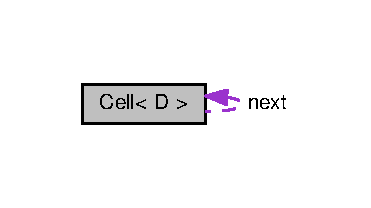
\includegraphics[width=178pt]{class_cell__coll__graph}
\end{center}
\end{figure}
\subsection*{Public Member Functions}
\begin{DoxyCompactItemize}
\item 
{\bf Cell} ()
\item 
{\bf Cell} (D $\ast$d, {\bf Cell} $\ast$c)
\item 
{\bfseries Cell} (const {\bf Cell} \&orig)\label{class_cell_a260a5d52d571c8d2f951d81df17154e2}

\end{DoxyCompactItemize}
\subsection*{Public Attributes}
\begin{DoxyCompactItemize}
\item 
{\bf Cell} $\ast$ {\bf next}\label{class_cell_a7e0e6c090f8aca70862c2dbc3257e3b9}

\begin{DoxyCompactList}\small\item\em Puntero que apunta a la celda siguiente. \end{DoxyCompactList}\item 
D $\ast$ {\bf data}\label{class_cell_ab8cc4d3059ef84a652eabc05b6c28f49}

\begin{DoxyCompactList}\small\item\em Puntero que apunta al dato almacenado en la celda. \end{DoxyCompactList}\end{DoxyCompactItemize}


\subsection{Detailed Description}
\subsubsection*{template$<$typename D$>$class Cell$<$ D $>$}

Plantilla de la clase Celda 

\subsection{Constructor \& Destructor Documentation}
\index{Cell@{Cell}!Cell@{Cell}}
\index{Cell@{Cell}!Cell@{Cell}}
\subsubsection[{Cell}]{\setlength{\rightskip}{0pt plus 5cm}template$<$typename D $>$ {\bf Cell}$<$ D $>$\-::{\bf Cell} (
\begin{DoxyParamCaption}
{}
\end{DoxyParamCaption}
)\hspace{0.3cm}{\ttfamily [inline]}}\label{class_cell_a742a2adf7fa420fa9cbe386a87b5c79b}
Constructor de la clase celda, sus atributos inician en nulo \index{Cell@{Cell}!Cell@{Cell}}
\index{Cell@{Cell}!Cell@{Cell}}
\subsubsection[{Cell}]{\setlength{\rightskip}{0pt plus 5cm}template$<$typename D $>$ {\bf Cell}$<$ D $>$\-::{\bf Cell} (
\begin{DoxyParamCaption}
\item[{D $\ast$}]{d, }
\item[{{\bf Cell}$<$ D $>$ $\ast$}]{c}
\end{DoxyParamCaption}
)\hspace{0.3cm}{\ttfamily [inline]}}\label{class_cell_aa8960323a8eeb23294419dd31349f18f}
Constructor de la clase celda, asigna a data y next, los valores recibidos como atributos 
\begin{DoxyParams}{Parameters}
{\em d} & puntero de tipo D \\
\hline
{\em c} & puntero de tipo \doxyref{Cell}{p.}{class_cell} \\
\hline
\end{DoxyParams}


The documentation for this class was generated from the following file\-:\begin{DoxyCompactItemize}
\item 
Cell.\-h\end{DoxyCompactItemize}

\section{Edge$<$ D $>$ Class Template Reference}
\label{class_edge}\index{Edge$<$ D $>$@{Edge$<$ D $>$}}


{\ttfamily \#include $<$Edge.\-h$>$}

\subsection*{Public Member Functions}
\begin{DoxyCompactItemize}
\item 
{\bf Edge} ()
\item 
{\bf Edge} (double w, {\bf Node}$<$ D $>$ $\ast$s, {\bf Node}$<$ D $>$ $\ast$d)
\item 
{\bf Edge} (const {\bf Edge}$<$ D $>$ \&orig)
\item 
virtual {\bf $\sim$\-Edge} ()
\end{DoxyCompactItemize}
\subsection*{Public Attributes}
\begin{DoxyCompactItemize}
\item 
{\bf Node}$<$ D $>$ $\ast$ {\bf predecessor}
\begin{DoxyCompactList}\small\item\em Puntero que indica el nodo de salida de la arista. \end{DoxyCompactList}\item 
{\bf Node}$<$ D $>$ $\ast$ {\bf successor}
\begin{DoxyCompactList}\small\item\em Puntero que indica el nodo de llegada de la arista. \end{DoxyCompactList}\item 
double {\bf weight}
\begin{DoxyCompactList}\small\item\em Atributo que corresponde al peso que toma de llegar del nodo de salida al nodo de llegada. \end{DoxyCompactList}\end{DoxyCompactItemize}


\subsection{Detailed Description}
\subsubsection*{template$<$typename D$>$class Edge$<$ D $>$}

Plantilla de la clase \doxyref{Edge}{p.}{class_edge} 

\subsection{Constructor \& Destructor Documentation}
\index{Edge@{Edge}!Edge@{Edge}}
\index{Edge@{Edge}!Edge@{Edge}}
\subsubsection[{Edge}]{\setlength{\rightskip}{0pt plus 5cm}template$<$typename D$>$ {\bf Edge}$<$ D $>$\-::{\bf Edge} (
\begin{DoxyParamCaption}
{}
\end{DoxyParamCaption}
)\hspace{0.3cm}{\ttfamily [inline]}}\label{class_edge_ad81f88d2a5cc93695d754baeb0918f75}
Constructor de la clase \doxyref{Edge}{p.}{class_edge}, inicializa sus atributos en nullptr \index{Edge@{Edge}!Edge@{Edge}}
\index{Edge@{Edge}!Edge@{Edge}}
\subsubsection[{Edge}]{\setlength{\rightskip}{0pt plus 5cm}template$<$typename D$>$ {\bf Edge}$<$ D $>$\-::{\bf Edge} (
\begin{DoxyParamCaption}
\item[{double}]{w, }
\item[{{\bf Node}$<$ D $>$ $\ast$}]{s, }
\item[{{\bf Node}$<$ D $>$ $\ast$}]{d}
\end{DoxyParamCaption}
)\hspace{0.3cm}{\ttfamily [inline]}}\label{class_edge_abcbefbc4c2c98c39b2b6c22ed8c5d197}
Constructor de la clase \doxyref{Edge}{p.}{class_edge}, inicializa sus atributos segun los valore enviados como parametros(w,s,d) 
\begin{DoxyParams}{Parameters}
{\em w} & weight \\
\hline
{\em s} & source \\
\hline
{\em d} & destiny \\
\hline
\end{DoxyParams}
\index{Edge@{Edge}!Edge@{Edge}}
\index{Edge@{Edge}!Edge@{Edge}}
\subsubsection[{Edge}]{\setlength{\rightskip}{0pt plus 5cm}template$<$typename D$>$ {\bf Edge}$<$ D $>$\-::{\bf Edge} (
\begin{DoxyParamCaption}
\item[{const {\bf Edge}$<$ D $>$ \&}]{orig}
\end{DoxyParamCaption}
)\hspace{0.3cm}{\ttfamily [inline]}}\label{class_edge_a476fcd35753f2375c3e5905e3a852d9c}
Constructor por copia \index{Edge@{Edge}!$\sim$\-Edge@{$\sim$\-Edge}}
\index{$\sim$\-Edge@{$\sim$\-Edge}!Edge@{Edge}}
\subsubsection[{$\sim$\-Edge}]{\setlength{\rightskip}{0pt plus 5cm}template$<$typename D$>$ virtual {\bf Edge}$<$ D $>$\-::$\sim${\bf Edge} (
\begin{DoxyParamCaption}
{}
\end{DoxyParamCaption}
)\hspace{0.3cm}{\ttfamily [inline]}, {\ttfamily [virtual]}}\label{class_edge_aa30e6627706a71f8b2d4f838fe15303c}
Destructor de la clase \doxyref{Edge}{p.}{class_edge} 

\subsection{Member Data Documentation}
\index{Edge@{Edge}!predecessor@{predecessor}}
\index{predecessor@{predecessor}!Edge@{Edge}}
\subsubsection[{predecessor}]{\setlength{\rightskip}{0pt plus 5cm}template$<$typename D$>$ {\bf Node}$<$D$>$$\ast$ {\bf Edge}$<$ D $>$\-::predecessor}\label{class_edge_afb8185528f4936a73ec3aa75df3a2da8}


Puntero que indica el nodo de salida de la arista. 

\index{Edge@{Edge}!successor@{successor}}
\index{successor@{successor}!Edge@{Edge}}
\subsubsection[{successor}]{\setlength{\rightskip}{0pt plus 5cm}template$<$typename D$>$ {\bf Node}$<$D$>$$\ast$ {\bf Edge}$<$ D $>$\-::successor}\label{class_edge_a40fca6983dee6c9631feafb8d41d0b10}


Puntero que indica el nodo de llegada de la arista. 

\index{Edge@{Edge}!weight@{weight}}
\index{weight@{weight}!Edge@{Edge}}
\subsubsection[{weight}]{\setlength{\rightskip}{0pt plus 5cm}template$<$typename D$>$ double {\bf Edge}$<$ D $>$\-::weight}\label{class_edge_a4147d8e7a5b7f44db4ffb6aed49ef569}


Atributo que corresponde al peso que toma de llegar del nodo de salida al nodo de llegada. 



The documentation for this class was generated from the following file\-:\begin{DoxyCompactItemize}
\item 
{\bf Edge.\-h}\end{DoxyCompactItemize}

\section{Graph\-With\-Pointer$<$ D $>$ Class Template Reference}
\label{class_graph_with_pointer}\index{Graph\-With\-Pointer$<$ D $>$@{Graph\-With\-Pointer$<$ D $>$}}
\subsection*{Public Member Functions}
\begin{DoxyCompactItemize}
\item 
{\bf Graph\-With\-Pointer} ()
\item 
void {\bf add\-Edge} (double w, {\bf Node}$<$ D $>$ $\ast$s, {\bf Node}$<$ D $>$ $\ast$d)
\item 
{\bf Node}$<$ D $>$ $\ast$ {\bf add\-Node} (D $\ast$d)
\item 
void {\bf del\-Edge} ({\bf Node}$<$ D $>$ $\ast$s, {\bf Node}$<$ D $>$ $\ast$d)
\item 
void {\bf del\-Node} (D $\ast$d)
\item 
{\bf Node}$<$ D $>$ $\ast$ {\bf first\-Node} ()
\item 
{\bf Node}$<$ D $>$ $\ast$ {\bf next\-Node} ({\bf Node}$<$ D $>$ t)
\item 
{\bf Node}$<$ D $>$ $\ast$ {\bf node} (int i)
\item 
D $\ast$ {\bf get\-Data} ({\bf Node}$<$ D $>$ $\ast$a)
\item 
{\bf Node}$<$ D $>$ $\ast$ {\bf dfs} (D $\ast$d)
\item 
{\bf Node}$<$ D $>$ $\ast$ {\bf bfs} (D $\ast$d)
\item 
int {\bf index} ({\bf Node}$<$ D $>$ $\ast$s)
\item 
double $\ast$ {\bf dijkstra} ({\bf Node}$<$ D $>$ $\ast$s)
\item 
double $\ast$$\ast$ {\bf floyd} ()
\item 
virtual {\bf $\sim$\-Graph\-With\-Pointer} ()
\end{DoxyCompactItemize}
\subsection*{Public Attributes}
\begin{DoxyCompactItemize}
\item 
{\bf Node}$<$ D $>$ $\ast$$\ast$ {\bf graph}\label{class_graph_with_pointer_aa0244d4abba9a569013bfeea80d8bdc8}

\begin{DoxyCompactList}\small\item\em Arreglo de tipo \doxyref{Node}{p.}{class_node} Pointer, donde se guardan los nodos que contiene el grafo. \end{DoxyCompactList}\item 
int {\bf num\-Nodes}\label{class_graph_with_pointer_a6385986823450390617bd282e1833d97}

\begin{DoxyCompactList}\small\item\em Atributo que indica la cantidad de nodos del grafo. \end{DoxyCompactList}\item 
int {\bf max\-Elements}\label{class_graph_with_pointer_a43179fee097cf66b2b6c28a8686c0b45}

\begin{DoxyCompactList}\small\item\em Atributo que indica la maxima cantidad de elementos que permite graph. \end{DoxyCompactList}\end{DoxyCompactItemize}


\subsection{Constructor \& Destructor Documentation}
\index{Graph\-With\-Pointer@{Graph\-With\-Pointer}!Graph\-With\-Pointer@{Graph\-With\-Pointer}}
\index{Graph\-With\-Pointer@{Graph\-With\-Pointer}!GraphWithPointer@{Graph\-With\-Pointer}}
\subsubsection[{Graph\-With\-Pointer}]{\setlength{\rightskip}{0pt plus 5cm}template$<$typename D $>$ {\bf Graph\-With\-Pointer}$<$ D $>$\-::{\bf Graph\-With\-Pointer} (
\begin{DoxyParamCaption}
{}
\end{DoxyParamCaption}
)\hspace{0.3cm}{\ttfamily [inline]}}\label{class_graph_with_pointer_a8934daf32ef649a0766f1c90d89746b2}
Constructor de la clase grafo. \index{Graph\-With\-Pointer@{Graph\-With\-Pointer}!$\sim$\-Graph\-With\-Pointer@{$\sim$\-Graph\-With\-Pointer}}
\index{$\sim$\-Graph\-With\-Pointer@{$\sim$\-Graph\-With\-Pointer}!GraphWithPointer@{Graph\-With\-Pointer}}
\subsubsection[{$\sim$\-Graph\-With\-Pointer}]{\setlength{\rightskip}{0pt plus 5cm}template$<$typename D $>$ virtual {\bf Graph\-With\-Pointer}$<$ D $>$\-::$\sim${\bf Graph\-With\-Pointer} (
\begin{DoxyParamCaption}
{}
\end{DoxyParamCaption}
)\hspace{0.3cm}{\ttfamily [inline]}, {\ttfamily [virtual]}}\label{class_graph_with_pointer_ad6a2f50c3f449b2d5afe5b1cf742d897}
Destructor de la clase \doxyref{Graph\-With\-Pointer}{p.}{class_graph_with_pointer} 

\subsection{Member Function Documentation}
\index{Graph\-With\-Pointer@{Graph\-With\-Pointer}!add\-Edge@{add\-Edge}}
\index{add\-Edge@{add\-Edge}!GraphWithPointer@{Graph\-With\-Pointer}}
\subsubsection[{add\-Edge}]{\setlength{\rightskip}{0pt plus 5cm}template$<$typename D $>$ void {\bf Graph\-With\-Pointer}$<$ D $>$\-::add\-Edge (
\begin{DoxyParamCaption}
\item[{double}]{w, }
\item[{{\bf Node}$<$ D $>$ $\ast$}]{s, }
\item[{{\bf Node}$<$ D $>$ $\ast$}]{d}
\end{DoxyParamCaption}
)\hspace{0.3cm}{\ttfamily [inline]}}\label{class_graph_with_pointer_a909e93ff72476f3372c0cb8bbfc87c8a}
add\-Edge, se agrega una arista a conexions del nodo s. 
\begin{DoxyParams}{Parameters}
{\em w} & peso \\
\hline
{\em s} & source \doxyref{Node}{p.}{class_node} \\
\hline
{\em d} & destiny \doxyref{Node}{p.}{class_node} \\
\hline
\end{DoxyParams}
\index{Graph\-With\-Pointer@{Graph\-With\-Pointer}!add\-Node@{add\-Node}}
\index{add\-Node@{add\-Node}!GraphWithPointer@{Graph\-With\-Pointer}}
\subsubsection[{add\-Node}]{\setlength{\rightskip}{0pt plus 5cm}template$<$typename D $>$ {\bf Node}$<$D$>$$\ast$ {\bf Graph\-With\-Pointer}$<$ D $>$\-::add\-Node (
\begin{DoxyParamCaption}
\item[{D $\ast$}]{d}
\end{DoxyParamCaption}
)\hspace{0.3cm}{\ttfamily [inline]}}\label{class_graph_with_pointer_a7c290766fe59a24e68f07e1eda3b6d1e}
add\-Node Agrega un nodo a graph 
\begin{DoxyParams}{Parameters}
{\em d} & dato que contendrá el nodo agregado. \\
\hline
\end{DoxyParams}
\index{Graph\-With\-Pointer@{Graph\-With\-Pointer}!bfs@{bfs}}
\index{bfs@{bfs}!GraphWithPointer@{Graph\-With\-Pointer}}
\subsubsection[{bfs}]{\setlength{\rightskip}{0pt plus 5cm}template$<$typename D $>$ {\bf Node}$<$D$>$$\ast$ {\bf Graph\-With\-Pointer}$<$ D $>$\-::bfs (
\begin{DoxyParamCaption}
\item[{D $\ast$}]{d}
\end{DoxyParamCaption}
)\hspace{0.3cm}{\ttfamily [inline]}}\label{class_graph_with_pointer_af1aaad8daf3aaf3a12873495db78c861}
Breadth first search La busqueda se comienza desde la raíz que es el primer vértice activo. En el siguiente paso se etiquetan como visitados todos los vecinos del vértice activo que no han sido etiquetados. Se continúa etiquetando todos los vecinos de los hijos de v que no hayan sido visitados aún. 
\begin{DoxyParams}{Parameters}
{\em d} & dato buscado. \\
\hline
\end{DoxyParams}
\begin{DoxyReturn}{Returns}
El nodo donde se ubica el dato. 

nullptr si el nodo no existe. 
\end{DoxyReturn}
\index{Graph\-With\-Pointer@{Graph\-With\-Pointer}!del\-Edge@{del\-Edge}}
\index{del\-Edge@{del\-Edge}!GraphWithPointer@{Graph\-With\-Pointer}}
\subsubsection[{del\-Edge}]{\setlength{\rightskip}{0pt plus 5cm}template$<$typename D $>$ void {\bf Graph\-With\-Pointer}$<$ D $>$\-::del\-Edge (
\begin{DoxyParamCaption}
\item[{{\bf Node}$<$ D $>$ $\ast$}]{s, }
\item[{{\bf Node}$<$ D $>$ $\ast$}]{d}
\end{DoxyParamCaption}
)\hspace{0.3cm}{\ttfamily [inline]}}\label{class_graph_with_pointer_ad1434f4f97b3b8f0bbddd67424fa25fa}
Elimina una arista de la lista de conexiones del nodo s. 
\begin{DoxyParams}{Parameters}
{\em s} & source node \\
\hline
{\em d} & destiny node \\
\hline
\end{DoxyParams}
\index{Graph\-With\-Pointer@{Graph\-With\-Pointer}!del\-Node@{del\-Node}}
\index{del\-Node@{del\-Node}!GraphWithPointer@{Graph\-With\-Pointer}}
\subsubsection[{del\-Node}]{\setlength{\rightskip}{0pt plus 5cm}template$<$typename D $>$ void {\bf Graph\-With\-Pointer}$<$ D $>$\-::del\-Node (
\begin{DoxyParamCaption}
\item[{D $\ast$}]{d}
\end{DoxyParamCaption}
)\hspace{0.3cm}{\ttfamily [inline]}}\label{class_graph_with_pointer_ae8a138fd63b1f3bf87dcab4394fc21d8}
Elimina el nodo que contiene al dato d de la lista graph. De manera que también elimina todas las aristas que lleguen a dicho nodo. 
\begin{DoxyParams}{Parameters}
{\em d} & dato que contiene el nodo que se desea borrar. \\
\hline
\end{DoxyParams}
\index{Graph\-With\-Pointer@{Graph\-With\-Pointer}!dfs@{dfs}}
\index{dfs@{dfs}!GraphWithPointer@{Graph\-With\-Pointer}}
\subsubsection[{dfs}]{\setlength{\rightskip}{0pt plus 5cm}template$<$typename D $>$ {\bf Node}$<$D$>$$\ast$ {\bf Graph\-With\-Pointer}$<$ D $>$\-::dfs (
\begin{DoxyParamCaption}
\item[{D $\ast$}]{d}
\end{DoxyParamCaption}
)\hspace{0.3cm}{\ttfamily [inline]}}\label{class_graph_with_pointer_a485589b0a3ea42b3f1936ef126bac3c8}
Depth first search. Recorre el grafo, desde su raíz y avanza de vértice en vértice, marcando cada vértice como visitado. La búsqueda siempre avanza hacia un vértice no marcado,internándose “profundamente” en el grafo sin repetir ningún vértice. Cuando se alcanza un vértice cuyos vecinos han sido marcados, se retrocede al anterior vértice visitado y se avanza desde éste. 
\begin{DoxyParams}{Parameters}
{\em d} & dato buscado \\
\hline
\end{DoxyParams}
\begin{DoxyReturn}{Returns}
El nodo dentro del grafo donde se ubica el dato. 

nullptr si el nodo que contenga al dato no existe 
\end{DoxyReturn}
\index{Graph\-With\-Pointer@{Graph\-With\-Pointer}!dijkstra@{dijkstra}}
\index{dijkstra@{dijkstra}!GraphWithPointer@{Graph\-With\-Pointer}}
\subsubsection[{dijkstra}]{\setlength{\rightskip}{0pt plus 5cm}template$<$typename D $>$ double$\ast$ {\bf Graph\-With\-Pointer}$<$ D $>$\-::dijkstra (
\begin{DoxyParamCaption}
\item[{{\bf Node}$<$ D $>$ $\ast$}]{s}
\end{DoxyParamCaption}
)\hspace{0.3cm}{\ttfamily [inline]}}\label{class_graph_with_pointer_a59e0c06c330024115a07e60dc5172b47}
Indica el peso correspondiente de ir de un nodo s, a cada uno de los nodos dentro del grafo 
\begin{DoxyParams}{Parameters}
{\em s} & source \doxyref{Node}{p.}{class_node} \\
\hline
\end{DoxyParams}
\begin{DoxyReturn}{Returns}
arreglo de tipo double. 
\end{DoxyReturn}
\index{Graph\-With\-Pointer@{Graph\-With\-Pointer}!first\-Node@{first\-Node}}
\index{first\-Node@{first\-Node}!GraphWithPointer@{Graph\-With\-Pointer}}
\subsubsection[{first\-Node}]{\setlength{\rightskip}{0pt plus 5cm}template$<$typename D $>$ {\bf Node}$<$D$>$$\ast$ {\bf Graph\-With\-Pointer}$<$ D $>$\-::first\-Node (
\begin{DoxyParamCaption}
{}
\end{DoxyParamCaption}
)\hspace{0.3cm}{\ttfamily [inline]}}\label{class_graph_with_pointer_afd7f08ef73c53d9629089ddf70bf3a83}
Indica el primer nodo que contiene graph. \begin{DoxyReturn}{Returns}
el primer nodo. 
\end{DoxyReturn}
\index{Graph\-With\-Pointer@{Graph\-With\-Pointer}!floyd@{floyd}}
\index{floyd@{floyd}!GraphWithPointer@{Graph\-With\-Pointer}}
\subsubsection[{floyd}]{\setlength{\rightskip}{0pt plus 5cm}template$<$typename D $>$ double$\ast$$\ast$ {\bf Graph\-With\-Pointer}$<$ D $>$\-::floyd (
\begin{DoxyParamCaption}
{}
\end{DoxyParamCaption}
)\hspace{0.3cm}{\ttfamily [inline]}}\label{class_graph_with_pointer_a525ca9513db45cfc310e3123104c2ae3}
Indica el peso que tiene de ir de cada uno de los nodos de graph, a los otros nodos pertenecientes a graph \begin{DoxyReturn}{Returns}
arreglo en 2\-D de doubles. 
\end{DoxyReturn}
\index{Graph\-With\-Pointer@{Graph\-With\-Pointer}!get\-Data@{get\-Data}}
\index{get\-Data@{get\-Data}!GraphWithPointer@{Graph\-With\-Pointer}}
\subsubsection[{get\-Data}]{\setlength{\rightskip}{0pt plus 5cm}template$<$typename D $>$ D$\ast$ {\bf Graph\-With\-Pointer}$<$ D $>$\-::get\-Data (
\begin{DoxyParamCaption}
\item[{{\bf Node}$<$ D $>$ $\ast$}]{a}
\end{DoxyParamCaption}
)\hspace{0.3cm}{\ttfamily [inline]}}\label{class_graph_with_pointer_ae8400a798378db62b2a610676930ea03}
Indica el dato que contiene un nodo 
\begin{DoxyParams}{Parameters}
{\em a} & Nodo \\
\hline
\end{DoxyParams}
\begin{DoxyReturn}{Returns}
dato que contiene a 
\end{DoxyReturn}
\index{Graph\-With\-Pointer@{Graph\-With\-Pointer}!index@{index}}
\index{index@{index}!GraphWithPointer@{Graph\-With\-Pointer}}
\subsubsection[{index}]{\setlength{\rightskip}{0pt plus 5cm}template$<$typename D $>$ int {\bf Graph\-With\-Pointer}$<$ D $>$\-::index (
\begin{DoxyParamCaption}
\item[{{\bf Node}$<$ D $>$ $\ast$}]{s}
\end{DoxyParamCaption}
)\hspace{0.3cm}{\ttfamily [inline]}}\label{class_graph_with_pointer_ade6891f46541a78c4ed580d8fcfb0414}
Indica la posicion dentro de graph donde se ubica el nodo s 
\begin{DoxyParams}{Parameters}
{\em s} & nodo \\
\hline
\end{DoxyParams}
\begin{DoxyReturn}{Returns}
posicion 
\end{DoxyReturn}
\index{Graph\-With\-Pointer@{Graph\-With\-Pointer}!next\-Node@{next\-Node}}
\index{next\-Node@{next\-Node}!GraphWithPointer@{Graph\-With\-Pointer}}
\subsubsection[{next\-Node}]{\setlength{\rightskip}{0pt plus 5cm}template$<$typename D $>$ {\bf Node}$<$D$>$$\ast$ {\bf Graph\-With\-Pointer}$<$ D $>$\-::next\-Node (
\begin{DoxyParamCaption}
\item[{{\bf Node}$<$ D $>$}]{t}
\end{DoxyParamCaption}
)\hspace{0.3cm}{\ttfamily [inline]}}\label{class_graph_with_pointer_aa9d671c4afa0c67f6b698d16182b77e8}
Indica el nodo que le sigue al nodo t. 
\begin{DoxyParams}{Parameters}
{\em t} & nodo \\
\hline
\end{DoxyParams}
\begin{DoxyReturn}{Returns}
el nodo siguiente a t 
\end{DoxyReturn}
\index{Graph\-With\-Pointer@{Graph\-With\-Pointer}!node@{node}}
\index{node@{node}!GraphWithPointer@{Graph\-With\-Pointer}}
\subsubsection[{node}]{\setlength{\rightskip}{0pt plus 5cm}template$<$typename D $>$ {\bf Node}$<$D$>$$\ast$ {\bf Graph\-With\-Pointer}$<$ D $>$\-::node (
\begin{DoxyParamCaption}
\item[{int}]{i}
\end{DoxyParamCaption}
)\hspace{0.3cm}{\ttfamily [inline]}}\label{class_graph_with_pointer_ad319cf428f15b976a20106ecb7404af8}
Indica el nodo que se encuentra en la posición i de graph 
\begin{DoxyParams}{Parameters}
{\em i} & posicion \\
\hline
\end{DoxyParams}
\begin{DoxyReturn}{Returns}
nodo que se encuentra en la posicion i de graph 
\end{DoxyReturn}


The documentation for this class was generated from the following file\-:\begin{DoxyCompactItemize}
\item 
Graph\-With\-Pointer.\-h\end{DoxyCompactItemize}

\hypertarget{class_list}{\section{Referencia de la plantilla de la Clase List$<$ D, P $>$}
\label{class_list}\index{List$<$ D, P $>$@{List$<$ D, P $>$}}
}


{\ttfamily \#include $<$List.\-h$>$}



Diagrama de herencias de List$<$ D, P $>$\nopagebreak
\begin{figure}[H]
\begin{center}
\leavevmode
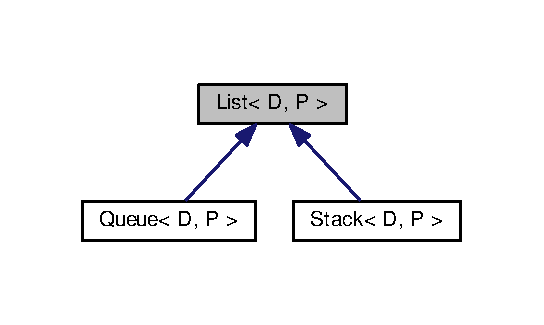
\includegraphics[width=202pt]{class_list__inherit__graph}
\end{center}
\end{figure}
\subsection*{Métodos públicos}
\begin{DoxyCompactItemize}
\item 
\hyperlink{class_list_a3deb54ab4f51c6c39aa4015f258b5812}{List} ()
\item 
\hyperlink{class_list_ad4d8108cecffb02dbc5e5e48691a0d43}{List} (int t)
\item 
\hyperlink{class_list_af8bcd7dae1bc30af2158075482c3d8d9}{List} (const \hyperlink{class_list}{List} \&orig)
\item 
virtual \hyperlink{class_list_a624593fb77847bf7ad4cacfba3442471}{$\sim$\-List} ()
\item 
virtual void \hyperlink{class_list_a01f588d87d47f8332928eca38f7b11bb}{insert} (D d)=0
\item 
virtual void \hyperlink{class_list_a14fc4e853102018df78db3899aa00d71}{remove} (D d)=0
\item 
virtual P \hyperlink{class_list_a2b40d6fffc7b2fb5138b648f52c839ee}{find} (D d)=0
\item 
virtual D \hyperlink{class_list_a5bd565e668247ae0691983227367cc88}{get} (P k)=0
\item 
virtual void \hyperlink{class_list_acb062aa988f4048498b30a2d845a311b}{assign} (P k, D d)=0
\item 
virtual void \hyperlink{class_list_ae3795939f27cf3e688cd470450e0c27a}{sort} ()=0
\item 
virtual int \hyperlink{class_list_af213bbcf13ee436a0f04cde66e337672}{get\-Size} ()=0
\item 
virtual void \hyperlink{class_list_a8b34931e187e7e6b86aad86510ce4f3b}{print\-List} ()=0
\item 
virtual P \hyperlink{class_list_a4ec3e88e176bb45bc49b030d1c8abb3f}{next} (P k)=0
\item 
virtual P \hyperlink{class_list_acc1831ae92a288345ef20cb29f3846b2}{prev} (P k)=0
\item 
virtual void \hyperlink{class_list_a24b4f177a70215980e81ef7b2981fa1e}{empty\-List} ()=0
\end{DoxyCompactItemize}


\subsection{Descripción detallada}
\subsubsection*{template$<$typename D, typename P$>$class List$<$ D, P $>$}

Plantilla de la clase \hyperlink{class_list}{List} 

\subsection{Documentación del constructor y destructor}
\hypertarget{class_list_a3deb54ab4f51c6c39aa4015f258b5812}{\index{List@{List}!List@{List}}
\index{List@{List}!List@{List}}
\subsubsection[{List}]{\setlength{\rightskip}{0pt plus 5cm}template$<$typename D, typename P$>$ {\bf List}$<$ D, P $>$\-::{\bf List} (
\begin{DoxyParamCaption}
{}
\end{DoxyParamCaption}
)\hspace{0.3cm}{\ttfamily [inline]}}}\label{class_list_a3deb54ab4f51c6c39aa4015f258b5812}
Constructor de la clase Lista sin atributos \hypertarget{class_list_ad4d8108cecffb02dbc5e5e48691a0d43}{\index{List@{List}!List@{List}}
\index{List@{List}!List@{List}}
\subsubsection[{List}]{\setlength{\rightskip}{0pt plus 5cm}template$<$typename D, typename P$>$ {\bf List}$<$ D, P $>$\-::{\bf List} (
\begin{DoxyParamCaption}
\item[{int}]{t}
\end{DoxyParamCaption}
)\hspace{0.3cm}{\ttfamily [inline]}}}\label{class_list_ad4d8108cecffb02dbc5e5e48691a0d43}
Constructor de la clase Lista. 
\begin{DoxyParams}{Parámetros}
{\em t} & tamaño de la lista \\
\hline
\end{DoxyParams}
\hypertarget{class_list_af8bcd7dae1bc30af2158075482c3d8d9}{\index{List@{List}!List@{List}}
\index{List@{List}!List@{List}}
\subsubsection[{List}]{\setlength{\rightskip}{0pt plus 5cm}template$<$typename D, typename P$>$ {\bf List}$<$ D, P $>$\-::{\bf List} (
\begin{DoxyParamCaption}
\item[{const {\bf List}$<$ D, P $>$ \&}]{orig}
\end{DoxyParamCaption}
)\hspace{0.3cm}{\ttfamily [inline]}}}\label{class_list_af8bcd7dae1bc30af2158075482c3d8d9}
Constructor por copia \hypertarget{class_list_a624593fb77847bf7ad4cacfba3442471}{\index{List@{List}!$\sim$\-List@{$\sim$\-List}}
\index{$\sim$\-List@{$\sim$\-List}!List@{List}}
\subsubsection[{$\sim$\-List}]{\setlength{\rightskip}{0pt plus 5cm}template$<$typename D, typename P$>$ virtual {\bf List}$<$ D, P $>$\-::$\sim${\bf List} (
\begin{DoxyParamCaption}
{}
\end{DoxyParamCaption}
)\hspace{0.3cm}{\ttfamily [inline]}, {\ttfamily [virtual]}}}\label{class_list_a624593fb77847bf7ad4cacfba3442471}
Destructor de la clase lista 

\subsection{Documentación de las funciones miembro}
\hypertarget{class_list_acb062aa988f4048498b30a2d845a311b}{\index{List@{List}!assign@{assign}}
\index{assign@{assign}!List@{List}}
\subsubsection[{assign}]{\setlength{\rightskip}{0pt plus 5cm}template$<$typename D, typename P$>$ virtual void {\bf List}$<$ D, P $>$\-::assign (
\begin{DoxyParamCaption}
\item[{P}]{k, }
\item[{D}]{d}
\end{DoxyParamCaption}
)\hspace{0.3cm}{\ttfamily [pure virtual]}}}\label{class_list_acb062aa988f4048498b30a2d845a311b}
Metodo virtual assign, asigna a una determinada posicion k, el valor d 
\begin{DoxyParams}{Parámetros}
{\em k} & dato tipo P, es una posicion o celda. \\
\hline
{\em d} & dado tipo D, que se quiere asignar a k \\
\hline
\end{DoxyParams}


Implementado en \hyperlink{class_list_with_pointer_aeaa834b22c4d7276a77ff29df3da7a30}{List\-With\-Pointer$<$ D, P $>$} y \hyperlink{class_list_with_pointer_aeaa834b22c4d7276a77ff29df3da7a30}{List\-With\-Pointer$<$ string, Cell$<$ string $>$ $\ast$ $>$}.

\hypertarget{class_list_a24b4f177a70215980e81ef7b2981fa1e}{\index{List@{List}!empty\-List@{empty\-List}}
\index{empty\-List@{empty\-List}!List@{List}}
\subsubsection[{empty\-List}]{\setlength{\rightskip}{0pt plus 5cm}template$<$typename D, typename P$>$ virtual void {\bf List}$<$ D, P $>$\-::empty\-List (
\begin{DoxyParamCaption}
{}
\end{DoxyParamCaption}
)\hspace{0.3cm}{\ttfamily [pure virtual]}}}\label{class_list_a24b4f177a70215980e81ef7b2981fa1e}
Metodo empty\-List, vacia la lista 

Implementado en \hyperlink{class_list_with_pointer_aec4f5374971962c79d397bbcd0080199}{List\-With\-Pointer$<$ D, P $>$} y \hyperlink{class_list_with_pointer_aec4f5374971962c79d397bbcd0080199}{List\-With\-Pointer$<$ string, Cell$<$ string $>$ $\ast$ $>$}.

\hypertarget{class_list_a2b40d6fffc7b2fb5138b648f52c839ee}{\index{List@{List}!find@{find}}
\index{find@{find}!List@{List}}
\subsubsection[{find}]{\setlength{\rightskip}{0pt plus 5cm}template$<$typename D, typename P$>$ virtual P {\bf List}$<$ D, P $>$\-::find (
\begin{DoxyParamCaption}
\item[{D}]{d}
\end{DoxyParamCaption}
)\hspace{0.3cm}{\ttfamily [pure virtual]}}}\label{class_list_a2b40d6fffc7b2fb5138b648f52c839ee}
Metodo virtual find, busca dentro de la lista el dato d. 
\begin{DoxyParams}{Parámetros}
{\em d} & dato tipo D que se desea encontrar. \\
\hline
\end{DoxyParams}
\begin{DoxyReturn}{Devuelve}
posicion o celda donde se encuentra el dato 
\end{DoxyReturn}


Implementado en \hyperlink{class_list_with_pointer_afeff8b963c197378553e2a3f73eaf66a}{List\-With\-Pointer$<$ D, P $>$} y \hyperlink{class_list_with_pointer_afeff8b963c197378553e2a3f73eaf66a}{List\-With\-Pointer$<$ string, Cell$<$ string $>$ $\ast$ $>$}.

\hypertarget{class_list_a5bd565e668247ae0691983227367cc88}{\index{List@{List}!get@{get}}
\index{get@{get}!List@{List}}
\subsubsection[{get}]{\setlength{\rightskip}{0pt plus 5cm}template$<$typename D, typename P$>$ virtual D {\bf List}$<$ D, P $>$\-::get (
\begin{DoxyParamCaption}
\item[{P}]{k}
\end{DoxyParamCaption}
)\hspace{0.3cm}{\ttfamily [pure virtual]}}}\label{class_list_a5bd565e668247ae0691983227367cc88}
Metodo virtual get, da el valor que se encuentra almacenado en la posicion k. 
\begin{DoxyParams}{Parámetros}
{\em k} & dato tipo P, es una posicion o celda. \\
\hline
\end{DoxyParams}
\begin{DoxyReturn}{Devuelve}
retorna el valor almacenado en k 
\end{DoxyReturn}


Implementado en \hyperlink{class_list_with_pointer_a0ff36c852334da8bc167356e636c1846}{List\-With\-Pointer$<$ D, P $>$} y \hyperlink{class_list_with_pointer_a0ff36c852334da8bc167356e636c1846}{List\-With\-Pointer$<$ string, Cell$<$ string $>$ $\ast$ $>$}.

\hypertarget{class_list_af213bbcf13ee436a0f04cde66e337672}{\index{List@{List}!get\-Size@{get\-Size}}
\index{get\-Size@{get\-Size}!List@{List}}
\subsubsection[{get\-Size}]{\setlength{\rightskip}{0pt plus 5cm}template$<$typename D, typename P$>$ virtual int {\bf List}$<$ D, P $>$\-::get\-Size (
\begin{DoxyParamCaption}
{}
\end{DoxyParamCaption}
)\hspace{0.3cm}{\ttfamily [pure virtual]}}}\label{class_list_af213bbcf13ee436a0f04cde66e337672}
Metodo virtual get\-Size, da el tamaño de la lista. \begin{DoxyReturn}{Devuelve}
el tamaño de la lista 
\end{DoxyReturn}


Implementado en \hyperlink{class_list_with_pointer_ac70c49b5703887fd867e90cdac3c706f}{List\-With\-Pointer$<$ D, P $>$} y \hyperlink{class_list_with_pointer_ac70c49b5703887fd867e90cdac3c706f}{List\-With\-Pointer$<$ string, Cell$<$ string $>$ $\ast$ $>$}.

\hypertarget{class_list_a01f588d87d47f8332928eca38f7b11bb}{\index{List@{List}!insert@{insert}}
\index{insert@{insert}!List@{List}}
\subsubsection[{insert}]{\setlength{\rightskip}{0pt plus 5cm}template$<$typename D, typename P$>$ virtual void {\bf List}$<$ D, P $>$\-::insert (
\begin{DoxyParamCaption}
\item[{D}]{d}
\end{DoxyParamCaption}
)\hspace{0.3cm}{\ttfamily [pure virtual]}}}\label{class_list_a01f588d87d47f8332928eca38f7b11bb}
Metodo virtual insert, agrega el dato d a la lista. 
\begin{DoxyParams}{Parámetros}
{\em d} & dato tipo D que se desea agregar a la lista \\
\hline
\end{DoxyParams}


Implementado en \hyperlink{class_list_with_pointer_a676e57683ade8e179e8eff5885f7309a}{List\-With\-Pointer$<$ D, P $>$} y \hyperlink{class_list_with_pointer_a676e57683ade8e179e8eff5885f7309a}{List\-With\-Pointer$<$ string, Cell$<$ string $>$ $\ast$ $>$}.

\hypertarget{class_list_a4ec3e88e176bb45bc49b030d1c8abb3f}{\index{List@{List}!next@{next}}
\index{next@{next}!List@{List}}
\subsubsection[{next}]{\setlength{\rightskip}{0pt plus 5cm}template$<$typename D, typename P$>$ virtual P {\bf List}$<$ D, P $>$\-::next (
\begin{DoxyParamCaption}
\item[{P}]{k}
\end{DoxyParamCaption}
)\hspace{0.3cm}{\ttfamily [pure virtual]}}}\label{class_list_a4ec3e88e176bb45bc49b030d1c8abb3f}
Metodo next, da la posicion o celda que le sigue a k 
\begin{DoxyParams}{Parámetros}
{\em k} & dato tipo P, es una posicion o celda. \\
\hline
\end{DoxyParams}
\begin{DoxyReturn}{Devuelve}
la posicion siguiente a k 
\end{DoxyReturn}


Implementado en \hyperlink{class_list_with_pointer_a518b5ee89e3ad32ae7cd4ddd5d4fa7e9}{List\-With\-Pointer$<$ D, P $>$} y \hyperlink{class_list_with_pointer_a518b5ee89e3ad32ae7cd4ddd5d4fa7e9}{List\-With\-Pointer$<$ string, Cell$<$ string $>$ $\ast$ $>$}.

\hypertarget{class_list_acc1831ae92a288345ef20cb29f3846b2}{\index{List@{List}!prev@{prev}}
\index{prev@{prev}!List@{List}}
\subsubsection[{prev}]{\setlength{\rightskip}{0pt plus 5cm}template$<$typename D, typename P$>$ virtual P {\bf List}$<$ D, P $>$\-::prev (
\begin{DoxyParamCaption}
\item[{P}]{k}
\end{DoxyParamCaption}
)\hspace{0.3cm}{\ttfamily [pure virtual]}}}\label{class_list_acc1831ae92a288345ef20cb29f3846b2}
Metodo next, retorna la posicion o celda que precede a k 
\begin{DoxyParams}{Parámetros}
{\em k} & dato tipo P, es una posicion o celda. \\
\hline
\end{DoxyParams}
\begin{DoxyReturn}{Devuelve}
la posicion previa a k 
\end{DoxyReturn}


Implementado en \hyperlink{class_list_with_pointer_a7242068fcc3a193f0f7e94517856e431}{List\-With\-Pointer$<$ D, P $>$} y \hyperlink{class_list_with_pointer_a7242068fcc3a193f0f7e94517856e431}{List\-With\-Pointer$<$ string, Cell$<$ string $>$ $\ast$ $>$}.

\hypertarget{class_list_a8b34931e187e7e6b86aad86510ce4f3b}{\index{List@{List}!print\-List@{print\-List}}
\index{print\-List@{print\-List}!List@{List}}
\subsubsection[{print\-List}]{\setlength{\rightskip}{0pt plus 5cm}template$<$typename D, typename P$>$ virtual void {\bf List}$<$ D, P $>$\-::print\-List (
\begin{DoxyParamCaption}
{}
\end{DoxyParamCaption}
)\hspace{0.3cm}{\ttfamily [pure virtual]}}}\label{class_list_a8b34931e187e7e6b86aad86510ce4f3b}
Metodo print\-List, imprime la lista 

Implementado en \hyperlink{class_list_with_pointer_a7079b5f1dbddb87a7e33ffc71ebb7b92}{List\-With\-Pointer$<$ D, P $>$} y \hyperlink{class_list_with_pointer_a7079b5f1dbddb87a7e33ffc71ebb7b92}{List\-With\-Pointer$<$ string, Cell$<$ string $>$ $\ast$ $>$}.

\hypertarget{class_list_a14fc4e853102018df78db3899aa00d71}{\index{List@{List}!remove@{remove}}
\index{remove@{remove}!List@{List}}
\subsubsection[{remove}]{\setlength{\rightskip}{0pt plus 5cm}template$<$typename D, typename P$>$ virtual void {\bf List}$<$ D, P $>$\-::remove (
\begin{DoxyParamCaption}
\item[{D}]{d}
\end{DoxyParamCaption}
)\hspace{0.3cm}{\ttfamily [pure virtual]}}}\label{class_list_a14fc4e853102018df78db3899aa00d71}
Metodo virtual remove , remueve el dato d de la lista, si este existe. 
\begin{DoxyParams}{Parámetros}
{\em d} & dato tipo D que se desea remover de la lista \\
\hline
\end{DoxyParams}


Implementado en \hyperlink{class_list_with_pointer_abcb151e95e9fffea7f9f7af593d8176f}{List\-With\-Pointer$<$ D, P $>$} y \hyperlink{class_list_with_pointer_abcb151e95e9fffea7f9f7af593d8176f}{List\-With\-Pointer$<$ string, Cell$<$ string $>$ $\ast$ $>$}.

\hypertarget{class_list_ae3795939f27cf3e688cd470450e0c27a}{\index{List@{List}!sort@{sort}}
\index{sort@{sort}!List@{List}}
\subsubsection[{sort}]{\setlength{\rightskip}{0pt plus 5cm}template$<$typename D, typename P$>$ virtual void {\bf List}$<$ D, P $>$\-::sort (
\begin{DoxyParamCaption}
{}
\end{DoxyParamCaption}
)\hspace{0.3cm}{\ttfamily [pure virtual]}}}\label{class_list_ae3795939f27cf3e688cd470450e0c27a}
Metodo virtual sort, ordena la lista 

Implementado en \hyperlink{class_list_with_pointer_aa46631b2da29895d1f767626fb591bc8}{List\-With\-Pointer$<$ D, P $>$} y \hyperlink{class_list_with_pointer_aa46631b2da29895d1f767626fb591bc8}{List\-With\-Pointer$<$ string, Cell$<$ string $>$ $\ast$ $>$}.



La documentación para esta clase fue generada a partir del siguiente fichero\-:\begin{DoxyCompactItemize}
\item 
List.\-h\end{DoxyCompactItemize}

\section{My\-Type Class Reference}
\label{class_my_type}\index{My\-Type@{My\-Type}}


Clase \doxyref{My\-Type}{p.}{class_my_type}.  




{\ttfamily \#include $<$My\-Type.\-h$>$}

\subsection*{Public Member Functions}
\begin{DoxyCompactItemize}
\item 
{\bf My\-Type} (char a)
\begin{DoxyCompactList}\small\item\em Constructor de la clase \doxyref{My\-Type}{p.}{class_my_type}. \end{DoxyCompactList}\item 
{\bf My\-Type} (const {\bf My\-Type} \&orig)
\begin{DoxyCompactList}\small\item\em Constructor por copia. \end{DoxyCompactList}\item 
virtual {\bf $\sim$\-My\-Type} ()
\begin{DoxyCompactList}\small\item\em Destructor de la clase \doxyref{My\-Type}{p.}{class_my_type}. \end{DoxyCompactList}\item 
bool {\bf operator==} (const {\bf My\-Type} \&other)
\item 
char {\bf operator$\ast$} ()
\end{DoxyCompactItemize}
\subsection*{Public Attributes}
\begin{DoxyCompactItemize}
\item 
char {\bf content}
\begin{DoxyCompactList}\small\item\em Atributo de la clase \doxyref{My\-Type}{p.}{class_my_type} que contiene un character. \end{DoxyCompactList}\end{DoxyCompactItemize}


\subsection{Detailed Description}
Clase \doxyref{My\-Type}{p.}{class_my_type}. 

Clase que tiene como atributo una variable de tipo char. 

\subsection{Constructor \& Destructor Documentation}
\index{My\-Type@{My\-Type}!My\-Type@{My\-Type}}
\index{My\-Type@{My\-Type}!MyType@{My\-Type}}
\subsubsection[{My\-Type}]{\setlength{\rightskip}{0pt plus 5cm}My\-Type\-::\-My\-Type (
\begin{DoxyParamCaption}
\item[{char}]{a}
\end{DoxyParamCaption}
)}\label{class_my_type_ad52b10cdc8bb9d9816b0fafa9dfe5cbc}


Constructor de la clase \doxyref{My\-Type}{p.}{class_my_type}. 


\begin{DoxyParams}{Parameters}
{\em a} & caracter que se le va a asignar al objeto\\
\hline
\end{DoxyParams}
Constructor de la clase \doxyref{My\-Type}{p.}{class_my_type}. Asigna el valor de a al atributo content. 
\begin{DoxyParams}{Parameters}
{\em a} & caracter que se desea que tenga el objeto \\
\hline
\end{DoxyParams}
\index{My\-Type@{My\-Type}!My\-Type@{My\-Type}}
\index{My\-Type@{My\-Type}!MyType@{My\-Type}}
\subsubsection[{My\-Type}]{\setlength{\rightskip}{0pt plus 5cm}My\-Type\-::\-My\-Type (
\begin{DoxyParamCaption}
\item[{const {\bf My\-Type} \&}]{orig}
\end{DoxyParamCaption}
)}\label{class_my_type_a2e1ca6579b32567672a5ba20a2f50f3f}


Constructor por copia. 

\index{My\-Type@{My\-Type}!$\sim$\-My\-Type@{$\sim$\-My\-Type}}
\index{$\sim$\-My\-Type@{$\sim$\-My\-Type}!MyType@{My\-Type}}
\subsubsection[{$\sim$\-My\-Type}]{\setlength{\rightskip}{0pt plus 5cm}My\-Type\-::$\sim$\-My\-Type (
\begin{DoxyParamCaption}
{}
\end{DoxyParamCaption}
)\hspace{0.3cm}{\ttfamily [virtual]}}\label{class_my_type_a887e8f9675b894dd43429173638c7ec5}


Destructor de la clase \doxyref{My\-Type}{p.}{class_my_type}. 

Destructor. 

\subsection{Member Function Documentation}
\index{My\-Type@{My\-Type}!operator$\ast$@{operator$\ast$}}
\index{operator$\ast$@{operator$\ast$}!MyType@{My\-Type}}
\subsubsection[{operator$\ast$}]{\setlength{\rightskip}{0pt plus 5cm}char My\-Type\-::operator$\ast$ (
\begin{DoxyParamCaption}
{}
\end{DoxyParamCaption}
)}\label{class_my_type_af2774d1abf8fe0f4434232b03230fea3}
Metodo que sobrecarga el operador $\ast$

Sobrecarga del operador $\ast$ \begin{DoxyReturn}{Returns}
el atributo content del objeto 
\end{DoxyReturn}
\index{My\-Type@{My\-Type}!operator==@{operator==}}
\index{operator==@{operator==}!MyType@{My\-Type}}
\subsubsection[{operator==}]{\setlength{\rightskip}{0pt plus 5cm}bool My\-Type\-::operator== (
\begin{DoxyParamCaption}
\item[{const {\bf My\-Type} \&}]{other}
\end{DoxyParamCaption}
)}\label{class_my_type_a7bb3a1722b97e644ea53de5618e47ad6}
Metodo que sobrecarga el operador ==

Sobrecarga del operador == \begin{DoxyReturn}{Returns}
true si los objetos son iguales 

false si los objetos son diferentes 
\end{DoxyReturn}


\subsection{Member Data Documentation}
\index{My\-Type@{My\-Type}!content@{content}}
\index{content@{content}!MyType@{My\-Type}}
\subsubsection[{content}]{\setlength{\rightskip}{0pt plus 5cm}char My\-Type\-::content}\label{class_my_type_a591d19d52f84c142e1dd21c5267b3c62}


Atributo de la clase \doxyref{My\-Type}{p.}{class_my_type} que contiene un character. 



The documentation for this class was generated from the following files\-:\begin{DoxyCompactItemize}
\item 
{\bf My\-Type.\-h}\item 
{\bf My\-Type.\-cpp}\end{DoxyCompactItemize}

\section{Node$<$ D $>$ Class Template Reference}
\label{class_node}\index{Node$<$ D $>$@{Node$<$ D $>$}}


{\ttfamily \#include $<$Node.\-h$>$}

\subsection*{Public Member Functions}
\begin{DoxyCompactItemize}
\item 
{\bf Node} ()
\begin{DoxyCompactList}\small\item\em Constructor de la clase \doxyref{Node}{p.}{class_node}, inicializa todos los atributos en nullptr o false, según corresponda. \end{DoxyCompactList}\item 
{\bf Node} (D $\ast$d)
\item 
void {\bf add\-Edge} ({\bf Edge}$<$ D $>$ d)
\item 
void {\bf del\-Edge} ({\bf Node}$<$ D $>$ $\ast$s, {\bf Node}$<$ D $>$ $\ast$d)
\item 
int $\ast$ {\bf search\-Edge} ({\bf Node}$<$ D $>$ $\ast$s, {\bf Node}$<$ D $>$ $\ast$d)
\item 
virtual {\bf $\sim$\-Node} ()
\begin{DoxyCompactList}\small\item\em Destructor de la clase \doxyref{Node}{p.}{class_node}. \end{DoxyCompactList}\end{DoxyCompactItemize}
\subsection*{Public Attributes}
\begin{DoxyCompactItemize}
\item 
D $\ast$ {\bf data}
\begin{DoxyCompactList}\small\item\em Atributo que tiene el dato almacenado en el nodo. \end{DoxyCompactList}\item 
{\bf Edge}$<$ D $>$ $\ast$ {\bf conexions}
\begin{DoxyCompactList}\small\item\em Arreglo que contiene todas las aristas que salen del nodo. \end{DoxyCompactList}\item 
int {\bf numconexions}
\begin{DoxyCompactList}\small\item\em Numero de aristas que tiene el nodo. \end{DoxyCompactList}\item 
int {\bf max\-Elements}
\begin{DoxyCompactList}\small\item\em Máxima cantidad de elementos que puede contener el arreglo conexions. \end{DoxyCompactList}\item 
bool {\bf been\-Here}
\begin{DoxyCompactList}\small\item\em Atributo de tipo bool que dice si se ha visitado el nodo. \end{DoxyCompactList}\item 
bool {\bf been\-Temp}
\begin{DoxyCompactList}\small\item\em Atributo de tipo bool, que indica si el nodo se ha utilizado para saber la distancia más corta entre un nodo y otro. \end{DoxyCompactList}\end{DoxyCompactItemize}


\subsection{Detailed Description}
\subsubsection*{template$<$typename D$>$class Node$<$ D $>$}

Plantilla de la clase \doxyref{Node}{p.}{class_node} 

\subsection{Constructor \& Destructor Documentation}
\index{Node@{Node}!Node@{Node}}
\index{Node@{Node}!Node@{Node}}
\subsubsection[{Node}]{\setlength{\rightskip}{0pt plus 5cm}template$<$typename D$>$ {\bf Node}$<$ D $>$\-::{\bf Node} (
\begin{DoxyParamCaption}
{}
\end{DoxyParamCaption}
)\hspace{0.3cm}{\ttfamily [inline]}}\label{class_node_a6d883b970cbbadb1f7d4785f737fc650}


Constructor de la clase \doxyref{Node}{p.}{class_node}, inicializa todos los atributos en nullptr o false, según corresponda. 

\index{Node@{Node}!Node@{Node}}
\index{Node@{Node}!Node@{Node}}
\subsubsection[{Node}]{\setlength{\rightskip}{0pt plus 5cm}template$<$typename D$>$ {\bf Node}$<$ D $>$\-::{\bf Node} (
\begin{DoxyParamCaption}
\item[{D $\ast$}]{d}
\end{DoxyParamCaption}
)\hspace{0.3cm}{\ttfamily [inline]}}\label{class_node_acae50cc855125df6d333368d28575b3e}
Constructor de la clase \doxyref{Node}{p.}{class_node}, inicializa data en d. 
\begin{DoxyParams}{Parameters}
{\em d} & dato de tipo puntero. \\
\hline
\end{DoxyParams}
\index{Node@{Node}!$\sim$\-Node@{$\sim$\-Node}}
\index{$\sim$\-Node@{$\sim$\-Node}!Node@{Node}}
\subsubsection[{$\sim$\-Node}]{\setlength{\rightskip}{0pt plus 5cm}template$<$typename D$>$ virtual {\bf Node}$<$ D $>$\-::$\sim${\bf Node} (
\begin{DoxyParamCaption}
{}
\end{DoxyParamCaption}
)\hspace{0.3cm}{\ttfamily [inline]}, {\ttfamily [virtual]}}\label{class_node_a6b5a080cf05afe6a81e4dd56ba5f90e3}


Destructor de la clase \doxyref{Node}{p.}{class_node}. 



\subsection{Member Function Documentation}
\index{Node@{Node}!add\-Edge@{add\-Edge}}
\index{add\-Edge@{add\-Edge}!Node@{Node}}
\subsubsection[{add\-Edge}]{\setlength{\rightskip}{0pt plus 5cm}template$<$typename D$>$ void {\bf Node}$<$ D $>$\-::add\-Edge (
\begin{DoxyParamCaption}
\item[{{\bf Edge}$<$ D $>$}]{d}
\end{DoxyParamCaption}
)\hspace{0.3cm}{\ttfamily [inline]}}\label{class_node_a3e6460cf5b82e6ede4cb1d2fba8ded16}
add\-Edge sirve para agregar aristas a la lista de aristas del nodo. 
\begin{DoxyParams}{Parameters}
{\em d} & objeto tipo arista. \\
\hline
\end{DoxyParams}
\index{Node@{Node}!del\-Edge@{del\-Edge}}
\index{del\-Edge@{del\-Edge}!Node@{Node}}
\subsubsection[{del\-Edge}]{\setlength{\rightskip}{0pt plus 5cm}template$<$typename D$>$ void {\bf Node}$<$ D $>$\-::del\-Edge (
\begin{DoxyParamCaption}
\item[{{\bf Node}$<$ D $>$ $\ast$}]{s, }
\item[{{\bf Node}$<$ D $>$ $\ast$}]{d}
\end{DoxyParamCaption}
)\hspace{0.3cm}{\ttfamily [inline]}}\label{class_node_a62e95e858c91952f7625e976114bbe8a}
del\-Edge remueve la arista que va de un nodo s al nodo d. 
\begin{DoxyParams}{Parameters}
{\em s} & Puntero que indica el nodo de partida. \\
\hline
{\em d} & Puntero que indica el nodo de llegada. \\
\hline
\end{DoxyParams}
\index{Node@{Node}!search\-Edge@{search\-Edge}}
\index{search\-Edge@{search\-Edge}!Node@{Node}}
\subsubsection[{search\-Edge}]{\setlength{\rightskip}{0pt plus 5cm}template$<$typename D$>$ int$\ast$ {\bf Node}$<$ D $>$\-::search\-Edge (
\begin{DoxyParamCaption}
\item[{{\bf Node}$<$ D $>$ $\ast$}]{s, }
\item[{{\bf Node}$<$ D $>$ $\ast$}]{d}
\end{DoxyParamCaption}
)\hspace{0.3cm}{\ttfamily [inline]}}\label{class_node_a0e0c1e71f6335ea4bf7c6dbbfdcca57e}
search\-Edge 
\begin{DoxyParams}{Parameters}
{\em s} & Puntero que indica el nodo de partida. \\
\hline
{\em d} & Puntero que indica el nodo de llegada. \\
\hline
\end{DoxyParams}
\begin{DoxyReturn}{Returns}
la posición dentro de conexions, donde se encuentra la arista solicitada 
\end{DoxyReturn}


\subsection{Member Data Documentation}
\index{Node@{Node}!been\-Here@{been\-Here}}
\index{been\-Here@{been\-Here}!Node@{Node}}
\subsubsection[{been\-Here}]{\setlength{\rightskip}{0pt plus 5cm}template$<$typename D$>$ bool {\bf Node}$<$ D $>$\-::been\-Here}\label{class_node_aac6afde6edec4fcb7be68c96666c1fe2}


Atributo de tipo bool que dice si se ha visitado el nodo. 

\index{Node@{Node}!been\-Temp@{been\-Temp}}
\index{been\-Temp@{been\-Temp}!Node@{Node}}
\subsubsection[{been\-Temp}]{\setlength{\rightskip}{0pt plus 5cm}template$<$typename D$>$ bool {\bf Node}$<$ D $>$\-::been\-Temp}\label{class_node_ad842fd061f930e3450a62c12ab93db24}


Atributo de tipo bool, que indica si el nodo se ha utilizado para saber la distancia más corta entre un nodo y otro. 

\index{Node@{Node}!conexions@{conexions}}
\index{conexions@{conexions}!Node@{Node}}
\subsubsection[{conexions}]{\setlength{\rightskip}{0pt plus 5cm}template$<$typename D$>$ {\bf Edge}$<$D$>$$\ast$ {\bf Node}$<$ D $>$\-::conexions}\label{class_node_abd882079b39e0674e0e9e50d2591d136}


Arreglo que contiene todas las aristas que salen del nodo. 

\index{Node@{Node}!data@{data}}
\index{data@{data}!Node@{Node}}
\subsubsection[{data}]{\setlength{\rightskip}{0pt plus 5cm}template$<$typename D$>$ D$\ast$ {\bf Node}$<$ D $>$\-::data}\label{class_node_a94c115991edeecf6664eaa4884fbf6ca}


Atributo que tiene el dato almacenado en el nodo. 

\index{Node@{Node}!max\-Elements@{max\-Elements}}
\index{max\-Elements@{max\-Elements}!Node@{Node}}
\subsubsection[{max\-Elements}]{\setlength{\rightskip}{0pt plus 5cm}template$<$typename D$>$ int {\bf Node}$<$ D $>$\-::max\-Elements}\label{class_node_a565fd8acc8938a43443f05c7c9e8d896}


Máxima cantidad de elementos que puede contener el arreglo conexions. 

\index{Node@{Node}!numconexions@{numconexions}}
\index{numconexions@{numconexions}!Node@{Node}}
\subsubsection[{numconexions}]{\setlength{\rightskip}{0pt plus 5cm}template$<$typename D$>$ int {\bf Node}$<$ D $>$\-::numconexions}\label{class_node_aa2f396eaa859fbd40a1b44950c0c539d}


Numero de aristas que tiene el nodo. 



The documentation for this class was generated from the following file\-:\begin{DoxyCompactItemize}
\item 
{\bf Node.\-h}\end{DoxyCompactItemize}

\section{Queue$<$ D, P $>$ Class Template Reference}
\label{class_queue}\index{Queue$<$ D, P $>$@{Queue$<$ D, P $>$}}


{\ttfamily \#include $<$Queue.\-h$>$}



Inheritance diagram for Queue$<$ D, P $>$\-:
\nopagebreak
\begin{figure}[H]
\begin{center}
\leavevmode
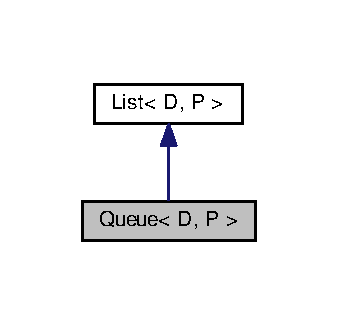
\includegraphics[width=162pt]{class_queue__inherit__graph}
\end{center}
\end{figure}


Collaboration diagram for Queue$<$ D, P $>$\-:
\nopagebreak
\begin{figure}[H]
\begin{center}
\leavevmode
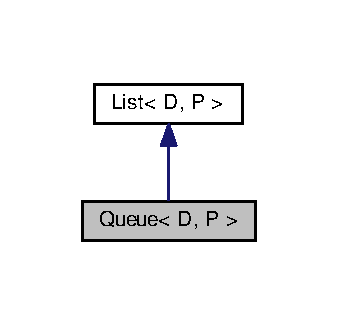
\includegraphics[width=162pt]{class_queue__coll__graph}
\end{center}
\end{figure}
\subsection*{Public Member Functions}
\begin{DoxyCompactItemize}
\item 
{\bf Queue} ()
\begin{DoxyCompactList}\small\item\em Constructor de la clase \doxyref{Queue}{p.}{class_queue}. \end{DoxyCompactList}\item 
virtual {\bf $\sim$\-Queue} ()
\begin{DoxyCompactList}\small\item\em Destructor de la clase \doxyref{Queue}{p.}{class_queue}. \end{DoxyCompactList}\item 
void {\bf insert} (D $\ast$d)
\begin{DoxyCompactList}\small\item\em Metodo de insercion de elementos a la cola. \end{DoxyCompactList}\item 
void {\bf remove} (D d)
\item 
P {\bf pop} ()
\item 
P {\bf find} (D d)
\item 
void {\bf assign} (P k, D d)
\item 
void {\bf sort} ()
\item 
int {\bf get\-Size} ()
\item 
void {\bf print\-List} ()
\item 
P {\bf next} (P k)
\item 
P {\bf prev} (P k)
\item 
D {\bf get} (P k)
\item 
void {\bf empty\-List} ()
\end{DoxyCompactItemize}
\subsection*{Public Attributes}
\begin{DoxyCompactItemize}
\item 
int {\bf n}
\begin{DoxyCompactList}\small\item\em Numero de elementos de la cola. \end{DoxyCompactList}\item 
P {\bf first}
\begin{DoxyCompactList}\small\item\em Puntero que apunta al primer elemento de la cola. \end{DoxyCompactList}\item 
P {\bf last}
\begin{DoxyCompactList}\small\item\em Puntero que apunta al último elemento de la cola. \end{DoxyCompactList}\end{DoxyCompactItemize}


\subsection{Detailed Description}
\subsubsection*{template$<$typename D, typename P$>$class Queue$<$ D, P $>$}

Plantilla de la clase Cola, que hereda de la clase Lista. 

\subsection{Constructor \& Destructor Documentation}
\index{Queue@{Queue}!Queue@{Queue}}
\index{Queue@{Queue}!Queue@{Queue}}
\subsubsection[{Queue}]{\setlength{\rightskip}{0pt plus 5cm}template$<$typename D, typename P$>$ {\bf Queue}$<$ D, P $>$\-::{\bf Queue} (
\begin{DoxyParamCaption}
{}
\end{DoxyParamCaption}
)\hspace{0.3cm}{\ttfamily [inline]}}\label{class_queue_aaecc8eba91905e5bda9752e0f85a150e}


Constructor de la clase \doxyref{Queue}{p.}{class_queue}. 

Constructor de una cola vacia \index{Queue@{Queue}!$\sim$\-Queue@{$\sim$\-Queue}}
\index{$\sim$\-Queue@{$\sim$\-Queue}!Queue@{Queue}}
\subsubsection[{$\sim$\-Queue}]{\setlength{\rightskip}{0pt plus 5cm}template$<$typename D, typename P$>$ virtual {\bf Queue}$<$ D, P $>$\-::$\sim${\bf Queue} (
\begin{DoxyParamCaption}
{}
\end{DoxyParamCaption}
)\hspace{0.3cm}{\ttfamily [inline]}, {\ttfamily [virtual]}}\label{class_queue_af88c0ebfc35932cdbbd75bae05e7a962}


Destructor de la clase \doxyref{Queue}{p.}{class_queue}. 

Llama al método empty\-List, para eliminar la cola. 

\subsection{Member Function Documentation}
\index{Queue@{Queue}!assign@{assign}}
\index{assign@{assign}!Queue@{Queue}}
\subsubsection[{assign}]{\setlength{\rightskip}{0pt plus 5cm}template$<$typename D, typename P$>$ void {\bf Queue}$<$ D, P $>$\-::assign (
\begin{DoxyParamCaption}
\item[{P}]{k, }
\item[{D}]{d}
\end{DoxyParamCaption}
)\hspace{0.3cm}{\ttfamily [inline]}, {\ttfamily [virtual]}}\label{class_queue_a81e1345ce465a07879f455fd1b6e086e}
Metodo assign, irrelevante para la cola 

Implements {\bf List$<$ D, P $>$} \doxyref{}{p.}{class_list_acb062aa988f4048498b30a2d845a311b}.

\index{Queue@{Queue}!empty\-List@{empty\-List}}
\index{empty\-List@{empty\-List}!Queue@{Queue}}
\subsubsection[{empty\-List}]{\setlength{\rightskip}{0pt plus 5cm}template$<$typename D, typename P$>$ void {\bf Queue}$<$ D, P $>$\-::empty\-List (
\begin{DoxyParamCaption}
{}
\end{DoxyParamCaption}
)\hspace{0.3cm}{\ttfamily [inline]}, {\ttfamily [virtual]}}\label{class_queue_a37e23ca9e4ac29be510833bf6b7f6638}
Metodo empty\-List, elimina todos los elementos pertenecientes a la cola. 

Implements {\bf List$<$ D, P $>$} \doxyref{}{p.}{class_list_a24b4f177a70215980e81ef7b2981fa1e}.

\index{Queue@{Queue}!find@{find}}
\index{find@{find}!Queue@{Queue}}
\subsubsection[{find}]{\setlength{\rightskip}{0pt plus 5cm}template$<$typename D, typename P$>$ P {\bf Queue}$<$ D, P $>$\-::find (
\begin{DoxyParamCaption}
\item[{D}]{d}
\end{DoxyParamCaption}
)\hspace{0.3cm}{\ttfamily [inline]}, {\ttfamily [virtual]}}\label{class_queue_a5c5ad7000d15506d3ec9c2ef6c8e6041}
Metodo find, irrelevante para la cola 

Implements {\bf List$<$ D, P $>$} \doxyref{}{p.}{class_list_a2b40d6fffc7b2fb5138b648f52c839ee}.

\index{Queue@{Queue}!get@{get}}
\index{get@{get}!Queue@{Queue}}
\subsubsection[{get}]{\setlength{\rightskip}{0pt plus 5cm}template$<$typename D, typename P$>$ D {\bf Queue}$<$ D, P $>$\-::get (
\begin{DoxyParamCaption}
\item[{P}]{k}
\end{DoxyParamCaption}
)\hspace{0.3cm}{\ttfamily [inline]}, {\ttfamily [virtual]}}\label{class_queue_a55cdbb6d999ef9a7a7afa5e39759701e}
Metodo get, irrelevante para la cola 

Implements {\bf List$<$ D, P $>$} \doxyref{}{p.}{class_list_a5bd565e668247ae0691983227367cc88}.

\index{Queue@{Queue}!get\-Size@{get\-Size}}
\index{get\-Size@{get\-Size}!Queue@{Queue}}
\subsubsection[{get\-Size}]{\setlength{\rightskip}{0pt plus 5cm}template$<$typename D, typename P$>$ int {\bf Queue}$<$ D, P $>$\-::get\-Size (
\begin{DoxyParamCaption}
{}
\end{DoxyParamCaption}
)\hspace{0.3cm}{\ttfamily [inline]}, {\ttfamily [virtual]}}\label{class_queue_ab2c7217e6737bf579493b321184a2db3}
Metodo get\-Size, da el tamaño de la cola. \begin{DoxyReturn}{Returns}
tamaño 
\end{DoxyReturn}


Implements {\bf List$<$ D, P $>$} \doxyref{}{p.}{class_list_af213bbcf13ee436a0f04cde66e337672}.

\index{Queue@{Queue}!insert@{insert}}
\index{insert@{insert}!Queue@{Queue}}
\subsubsection[{insert}]{\setlength{\rightskip}{0pt plus 5cm}template$<$typename D, typename P$>$ void {\bf Queue}$<$ D, P $>$\-::insert (
\begin{DoxyParamCaption}
\item[{D $\ast$}]{d}
\end{DoxyParamCaption}
)\hspace{0.3cm}{\ttfamily [inline]}, {\ttfamily [virtual]}}\label{class_queue_a3f3767b13bbd1a688dd13eb0fd8880c0}


Metodo de insercion de elementos a la cola. 

Dichos elementos solo pueden ser ingresados al final de la cola. Si la cola esta vacia, al insertar el elemento, este tendra los punteros first y last apuntando a él. De lo contrario, se crea la conexión entre el penúltimo elemento y el elemento agregado, y el puntero last apuntará a este elemento. 
\begin{DoxyParams}{Parameters}
{\em d} & dato tipo D que será ingresado a la cola. \\
\hline
\end{DoxyParams}


Implements {\bf List$<$ D, P $>$} \doxyref{}{p.}{class_list_a750822c0f61577bfb5297ea44aebe5a8}.

\index{Queue@{Queue}!next@{next}}
\index{next@{next}!Queue@{Queue}}
\subsubsection[{next}]{\setlength{\rightskip}{0pt plus 5cm}template$<$typename D, typename P$>$ P {\bf Queue}$<$ D, P $>$\-::next (
\begin{DoxyParamCaption}
\item[{P}]{k}
\end{DoxyParamCaption}
)\hspace{0.3cm}{\ttfamily [inline]}, {\ttfamily [virtual]}}\label{class_queue_aa4c9b83f260a172e1fffc389f354386f}
Metodo next, irrelevante para la cola 

Implements {\bf List$<$ D, P $>$} \doxyref{}{p.}{class_list_a4ec3e88e176bb45bc49b030d1c8abb3f}.

\index{Queue@{Queue}!pop@{pop}}
\index{pop@{pop}!Queue@{Queue}}
\subsubsection[{pop}]{\setlength{\rightskip}{0pt plus 5cm}template$<$typename D, typename P$>$ P {\bf Queue}$<$ D, P $>$\-::pop (
\begin{DoxyParamCaption}
{}
\end{DoxyParamCaption}
)\hspace{0.3cm}{\ttfamily [inline]}}\label{class_queue_aabf479754d981d43cebf7e8e68225881}
\index{Queue@{Queue}!prev@{prev}}
\index{prev@{prev}!Queue@{Queue}}
\subsubsection[{prev}]{\setlength{\rightskip}{0pt plus 5cm}template$<$typename D, typename P$>$ P {\bf Queue}$<$ D, P $>$\-::prev (
\begin{DoxyParamCaption}
\item[{P}]{k}
\end{DoxyParamCaption}
)\hspace{0.3cm}{\ttfamily [inline]}, {\ttfamily [virtual]}}\label{class_queue_adcb9a0e709ea65bc7e98f7e9cbae8a39}
Metodo prev, irrelevante para la cola 

Implements {\bf List$<$ D, P $>$} \doxyref{}{p.}{class_list_acc1831ae92a288345ef20cb29f3846b2}.

\index{Queue@{Queue}!print\-List@{print\-List}}
\index{print\-List@{print\-List}!Queue@{Queue}}
\subsubsection[{print\-List}]{\setlength{\rightskip}{0pt plus 5cm}template$<$typename D, typename P$>$ void {\bf Queue}$<$ D, P $>$\-::print\-List (
\begin{DoxyParamCaption}
{}
\end{DoxyParamCaption}
)\hspace{0.3cm}{\ttfamily [inline]}, {\ttfamily [virtual]}}\label{class_queue_aa461f8fb363f960a6e0eb34b18503eaa}
Metodo print\-List, imprime la cola 

Implements {\bf List$<$ D, P $>$} \doxyref{}{p.}{class_list_a8b34931e187e7e6b86aad86510ce4f3b}.

\index{Queue@{Queue}!remove@{remove}}
\index{remove@{remove}!Queue@{Queue}}
\subsubsection[{remove}]{\setlength{\rightskip}{0pt plus 5cm}template$<$typename D, typename P$>$ void {\bf Queue}$<$ D, P $>$\-::remove (
\begin{DoxyParamCaption}
\item[{D}]{d}
\end{DoxyParamCaption}
)\hspace{0.3cm}{\ttfamily [inline]}, {\ttfamily [virtual]}}\label{class_queue_a554993da9edb157443b0d956f11c8354}
Metodo que remueve el ultimo elemento de la cola. 
\begin{DoxyParams}{Parameters}
{\em d} & dato tipo D. Irrelevante para la cola. \\
\hline
\end{DoxyParams}


Implements {\bf List$<$ D, P $>$} \doxyref{}{p.}{class_list_a14fc4e853102018df78db3899aa00d71}.

\index{Queue@{Queue}!sort@{sort}}
\index{sort@{sort}!Queue@{Queue}}
\subsubsection[{sort}]{\setlength{\rightskip}{0pt plus 5cm}template$<$typename D, typename P$>$ void {\bf Queue}$<$ D, P $>$\-::sort (
\begin{DoxyParamCaption}
{}
\end{DoxyParamCaption}
)\hspace{0.3cm}{\ttfamily [inline]}, {\ttfamily [virtual]}}\label{class_queue_a896b0e1bcac0d660079eb838c1823446}
Metodo sort, irrelevante para la cola 

Implements {\bf List$<$ D, P $>$} \doxyref{}{p.}{class_list_ae3795939f27cf3e688cd470450e0c27a}.



\subsection{Member Data Documentation}
\index{Queue@{Queue}!first@{first}}
\index{first@{first}!Queue@{Queue}}
\subsubsection[{first}]{\setlength{\rightskip}{0pt plus 5cm}template$<$typename D, typename P$>$ P {\bf Queue}$<$ D, P $>$\-::first}\label{class_queue_a66d3f4dcd98ff256982192ccd4cbe1d4}


Puntero que apunta al primer elemento de la cola. 

\index{Queue@{Queue}!last@{last}}
\index{last@{last}!Queue@{Queue}}
\subsubsection[{last}]{\setlength{\rightskip}{0pt plus 5cm}template$<$typename D, typename P$>$ P {\bf Queue}$<$ D, P $>$\-::last}\label{class_queue_a8fa09b42d16c1fe9dea414b29ab9612f}


Puntero que apunta al último elemento de la cola. 

\index{Queue@{Queue}!n@{n}}
\index{n@{n}!Queue@{Queue}}
\subsubsection[{n}]{\setlength{\rightskip}{0pt plus 5cm}template$<$typename D, typename P$>$ int {\bf Queue}$<$ D, P $>$\-::n}\label{class_queue_a2b095618e827a9e728cb843bf4c0919e}


Numero de elementos de la cola. 



The documentation for this class was generated from the following file\-:\begin{DoxyCompactItemize}
\item 
{\bf Queue.\-h}\end{DoxyCompactItemize}

\section{Stack$<$ D, P $>$ Class Template Reference}
\label{class_stack}\index{Stack$<$ D, P $>$@{Stack$<$ D, P $>$}}


{\ttfamily \#include $<$Stack.\-h$>$}



Inheritance diagram for Stack$<$ D, P $>$\-:
\nopagebreak
\begin{figure}[H]
\begin{center}
\leavevmode
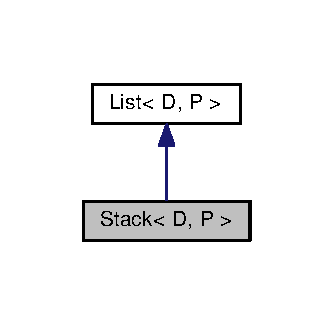
\includegraphics[width=160pt]{class_stack__inherit__graph}
\end{center}
\end{figure}


Collaboration diagram for Stack$<$ D, P $>$\-:
\nopagebreak
\begin{figure}[H]
\begin{center}
\leavevmode
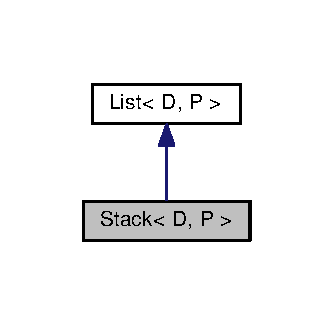
\includegraphics[width=160pt]{class_stack__coll__graph}
\end{center}
\end{figure}
\subsection*{Public Member Functions}
\begin{DoxyCompactItemize}
\item 
{\bf Stack} ()
\begin{DoxyCompactList}\small\item\em Constructor \doxyref{Stack}{p.}{class_stack}. \end{DoxyCompactList}\item 
void {\bf insert} (D $\ast$d)
\begin{DoxyCompactList}\small\item\em Metodo Insert. \end{DoxyCompactList}\item 
void {\bf remove} (D d)
\begin{DoxyCompactList}\small\item\em Metodo remove. \end{DoxyCompactList}\item 
void {\bf pop} ()
\item 
P {\bf find} (D d)
\item 
void {\bf assign} (P k, D d)
\item 
void {\bf sort} ()
\item 
int {\bf get\-Size} ()
\begin{DoxyCompactList}\small\item\em Metodo get\-Size. \end{DoxyCompactList}\item 
void {\bf print\-List} ()
\begin{DoxyCompactList}\small\item\em Metodo print\-List. \end{DoxyCompactList}\item 
P {\bf next} (P k)
\item 
P {\bf prev} (P k)
\begin{DoxyCompactList}\small\item\em Metodo prev. \end{DoxyCompactList}\item 
D {\bf get} (P k)
\item 
void {\bf empty\-List} ()
\end{DoxyCompactItemize}
\subsection*{Public Attributes}
\begin{DoxyCompactItemize}
\item 
int {\bf n}
\item 
P {\bf first}
\item 
P {\bf last}
\end{DoxyCompactItemize}


\subsection{Constructor \& Destructor Documentation}
\index{Stack@{Stack}!Stack@{Stack}}
\index{Stack@{Stack}!Stack@{Stack}}
\subsubsection[{Stack}]{\setlength{\rightskip}{0pt plus 5cm}template$<$typename D, typename P$>$ {\bf Stack}$<$ D, P $>$\-::{\bf Stack} (
\begin{DoxyParamCaption}
{}
\end{DoxyParamCaption}
)\hspace{0.3cm}{\ttfamily [inline]}}\label{class_stack_a6e0f84830cde41cb8d49818842d18d36}


Constructor \doxyref{Stack}{p.}{class_stack}. 

Crea el objeto tipo \doxyref{Stack}{p.}{class_stack}. 
\begin{DoxyParams}{Parameters}
{\em first} & es un puntero a la primera celda de la pila. \\
\hline
{\em last} & es un puntero a la ultima celda de la pila. \\
\hline
{\em n} & es la cantidad de elementos en la pila. \\
\hline
\end{DoxyParams}


\subsection{Member Function Documentation}
\index{Stack@{Stack}!assign@{assign}}
\index{assign@{assign}!Stack@{Stack}}
\subsubsection[{assign}]{\setlength{\rightskip}{0pt plus 5cm}template$<$typename D, typename P$>$ void {\bf Stack}$<$ D, P $>$\-::assign (
\begin{DoxyParamCaption}
\item[{P}]{k, }
\item[{D}]{d}
\end{DoxyParamCaption}
)\hspace{0.3cm}{\ttfamily [inline]}, {\ttfamily [virtual]}}\label{class_stack_ad36bacdff9f82a8718559606b46b145c}
Metodo virtual assign, asigna a una determinada posicion k, el valor d 
\begin{DoxyParams}{Parameters}
{\em k} & dato tipo P, es una posicion o celda. \\
\hline
{\em d} & dado tipo D, que se quiere asignar a k \\
\hline
\end{DoxyParams}


Implements {\bf List$<$ D, P $>$} \doxyref{}{p.}{class_list_acb062aa988f4048498b30a2d845a311b}.

\index{Stack@{Stack}!empty\-List@{empty\-List}}
\index{empty\-List@{empty\-List}!Stack@{Stack}}
\subsubsection[{empty\-List}]{\setlength{\rightskip}{0pt plus 5cm}template$<$typename D, typename P$>$ void {\bf Stack}$<$ D, P $>$\-::empty\-List (
\begin{DoxyParamCaption}
{}
\end{DoxyParamCaption}
)\hspace{0.3cm}{\ttfamily [inline]}, {\ttfamily [virtual]}}\label{class_stack_a8d4119c8d4be2822f20a525743aa296e}
Metodo empty\-List, vacia la lista 

Implements {\bf List$<$ D, P $>$} \doxyref{}{p.}{class_list_a24b4f177a70215980e81ef7b2981fa1e}.

\index{Stack@{Stack}!find@{find}}
\index{find@{find}!Stack@{Stack}}
\subsubsection[{find}]{\setlength{\rightskip}{0pt plus 5cm}template$<$typename D, typename P$>$ P {\bf Stack}$<$ D, P $>$\-::find (
\begin{DoxyParamCaption}
\item[{D}]{d}
\end{DoxyParamCaption}
)\hspace{0.3cm}{\ttfamily [inline]}, {\ttfamily [virtual]}}\label{class_stack_aa8a3a0b773900e44f641e3be9d9345da}
Metodo virtual find, busca dentro de la lista el dato d. 
\begin{DoxyParams}{Parameters}
{\em d} & dato tipo D que se desea encontrar. \\
\hline
\end{DoxyParams}
\begin{DoxyReturn}{Returns}
posicion o celda donde se encuentra el dato 
\end{DoxyReturn}


Implements {\bf List$<$ D, P $>$} \doxyref{}{p.}{class_list_a2b40d6fffc7b2fb5138b648f52c839ee}.

\index{Stack@{Stack}!get@{get}}
\index{get@{get}!Stack@{Stack}}
\subsubsection[{get}]{\setlength{\rightskip}{0pt plus 5cm}template$<$typename D, typename P$>$ D {\bf Stack}$<$ D, P $>$\-::get (
\begin{DoxyParamCaption}
\item[{P}]{k}
\end{DoxyParamCaption}
)\hspace{0.3cm}{\ttfamily [inline]}, {\ttfamily [virtual]}}\label{class_stack_a64eaffbf031ad032772e802ec88378df}
Metodo virtual get, da el valor que se encuentra almacenado en la posicion k. 
\begin{DoxyParams}{Parameters}
{\em k} & dato tipo P, es una posicion o celda. \\
\hline
\end{DoxyParams}
\begin{DoxyReturn}{Returns}
retorna el valor almacenado en k 
\end{DoxyReturn}


Implements {\bf List$<$ D, P $>$} \doxyref{}{p.}{class_list_a5bd565e668247ae0691983227367cc88}.

\index{Stack@{Stack}!get\-Size@{get\-Size}}
\index{get\-Size@{get\-Size}!Stack@{Stack}}
\subsubsection[{get\-Size}]{\setlength{\rightskip}{0pt plus 5cm}template$<$typename D, typename P$>$ int {\bf Stack}$<$ D, P $>$\-::get\-Size (
\begin{DoxyParamCaption}
{}
\end{DoxyParamCaption}
)\hspace{0.3cm}{\ttfamily [inline]}, {\ttfamily [virtual]}}\label{class_stack_a74fc7e5921dfb247f9ad7052c3c4297a}


Metodo get\-Size. 

Retorna la cantidad de elementos de la pila. \begin{DoxyReturn}{Returns}
n, es posible determinar el tamaño de la pila con el atributo n. 
\end{DoxyReturn}


Implements {\bf List$<$ D, P $>$} \doxyref{}{p.}{class_list_af213bbcf13ee436a0f04cde66e337672}.

\index{Stack@{Stack}!insert@{insert}}
\index{insert@{insert}!Stack@{Stack}}
\subsubsection[{insert}]{\setlength{\rightskip}{0pt plus 5cm}template$<$typename D, typename P$>$ void {\bf Stack}$<$ D, P $>$\-::insert (
\begin{DoxyParamCaption}
\item[{D $\ast$}]{d}
\end{DoxyParamCaption}
)\hspace{0.3cm}{\ttfamily [inline]}, {\ttfamily [virtual]}}\label{class_stack_afed02ed90b717dc8e34daf02e2d3b586}


Metodo Insert. 

Inserta un elemento a la pila. Se crea un objeto newest tipo celda, que almacena al dato d. En caso de que la pila este vacia, se almacena esta celda creada en los punteros last y first . En caso de que la pila no este vacia, se realiza la coneccion de manera que ahora la ultima celda se convierta en la penultima(apuntando a la ultima). Se suma 1 a la cantidad de elementos. 
\begin{DoxyParams}{Parameters}
{\em d} & es un dato tipo D que se desea insertar en la pila. \\
\hline
{\em newest} & es un objeto tipo P. \\
\hline
\end{DoxyParams}


Implements {\bf List$<$ D, P $>$} \doxyref{}{p.}{class_list_a750822c0f61577bfb5297ea44aebe5a8}.

\index{Stack@{Stack}!next@{next}}
\index{next@{next}!Stack@{Stack}}
\subsubsection[{next}]{\setlength{\rightskip}{0pt plus 5cm}template$<$typename D, typename P$>$ P {\bf Stack}$<$ D, P $>$\-::next (
\begin{DoxyParamCaption}
\item[{P}]{k}
\end{DoxyParamCaption}
)\hspace{0.3cm}{\ttfamily [inline]}, {\ttfamily [virtual]}}\label{class_stack_ab7f8f7e4ab10c00769c1debc5391fc17}
Metodo next, da la posicion o celda que le sigue a k 
\begin{DoxyParams}{Parameters}
{\em k} & dato tipo P, es una posicion o celda. \\
\hline
\end{DoxyParams}
\begin{DoxyReturn}{Returns}
la posicion siguiente a k 
\end{DoxyReturn}


Implements {\bf List$<$ D, P $>$} \doxyref{}{p.}{class_list_a4ec3e88e176bb45bc49b030d1c8abb3f}.

\index{Stack@{Stack}!pop@{pop}}
\index{pop@{pop}!Stack@{Stack}}
\subsubsection[{pop}]{\setlength{\rightskip}{0pt plus 5cm}template$<$typename D, typename P$>$ void {\bf Stack}$<$ D, P $>$\-::pop (
\begin{DoxyParamCaption}
{}
\end{DoxyParamCaption}
)\hspace{0.3cm}{\ttfamily [inline]}}\label{class_stack_a9b465ba5e1c0be277775755dd680e52d}
\index{Stack@{Stack}!prev@{prev}}
\index{prev@{prev}!Stack@{Stack}}
\subsubsection[{prev}]{\setlength{\rightskip}{0pt plus 5cm}template$<$typename D, typename P$>$ P {\bf Stack}$<$ D, P $>$\-::prev (
\begin{DoxyParamCaption}
\item[{P}]{k}
\end{DoxyParamCaption}
)\hspace{0.3cm}{\ttfamily [inline]}, {\ttfamily [virtual]}}\label{class_stack_a0c0b55f72c9249bfb9252bce1a93458d}


Metodo prev. 

Para una pila este metodo no tiene sentido, sin embargo es util para otros metodos de la clase. Este metodo recibe un puntero a un objeto tipo \doxyref{Cell}{p.}{class_cell}, y recorre toda la pila(tal como una lista), buscando que celda apunta a la celda indicada, a partir del atributo next. 
\begin{DoxyParams}{Parameters}
{\em k} & es un puntero a un objeto tipo \doxyref{Cell}{p.}{class_cell}. \\
\hline
\end{DoxyParams}
\begin{DoxyReturn}{Returns}
retorna un puntero a la celda previa si se encontro, caso contrario retorna un nullptr 
\end{DoxyReturn}


Implements {\bf List$<$ D, P $>$} \doxyref{}{p.}{class_list_acc1831ae92a288345ef20cb29f3846b2}.

\index{Stack@{Stack}!print\-List@{print\-List}}
\index{print\-List@{print\-List}!Stack@{Stack}}
\subsubsection[{print\-List}]{\setlength{\rightskip}{0pt plus 5cm}template$<$typename D, typename P$>$ void {\bf Stack}$<$ D, P $>$\-::print\-List (
\begin{DoxyParamCaption}
{}
\end{DoxyParamCaption}
)\hspace{0.3cm}{\ttfamily [inline]}, {\ttfamily [virtual]}}\label{class_stack_a89b9967c15c83fe7c257a42e49725881}


Metodo print\-List. 

Imprime la pila. La pila se ve en pantalla en orden descendente, donde los elementos que se agregan a la pila van abajo. Y por lo tanto es de abajo que se tienen que extraer los valores. Se imprime como si fuese una lista, recorriendo todos sus elementos e imprimiendo el dato correspondiente a cada elemento. 

Implements {\bf List$<$ D, P $>$} \doxyref{}{p.}{class_list_a8b34931e187e7e6b86aad86510ce4f3b}.

\index{Stack@{Stack}!remove@{remove}}
\index{remove@{remove}!Stack@{Stack}}
\subsubsection[{remove}]{\setlength{\rightskip}{0pt plus 5cm}template$<$typename D, typename P$>$ void {\bf Stack}$<$ D, P $>$\-::remove (
\begin{DoxyParamCaption}
\item[{D}]{d}
\end{DoxyParamCaption}
)\hspace{0.3cm}{\ttfamily [inline]}, {\ttfamily [virtual]}}\label{class_stack_a55637a6d0aed4283776ce2d159c3a58b}


Metodo remove. 

Remueve un elemento de la pila. Al ser una pila, se sigue un orden L\-I\-F\-O(\-Last In First Out) Basicamente se asigna la penultima posicion de la pila como la ultima, descartando el elemento que ingreso a la pila mas recientemente. Se resta 1 a la cantidad de elementos. 

Implements {\bf List$<$ D, P $>$} \doxyref{}{p.}{class_list_a14fc4e853102018df78db3899aa00d71}.

\index{Stack@{Stack}!sort@{sort}}
\index{sort@{sort}!Stack@{Stack}}
\subsubsection[{sort}]{\setlength{\rightskip}{0pt plus 5cm}template$<$typename D, typename P$>$ void {\bf Stack}$<$ D, P $>$\-::sort (
\begin{DoxyParamCaption}
{}
\end{DoxyParamCaption}
)\hspace{0.3cm}{\ttfamily [inline]}, {\ttfamily [virtual]}}\label{class_stack_a75261d2340f1f7b5e61b3770c0550982}
Metodo virtual sort, ordena la lista 

Implements {\bf List$<$ D, P $>$} \doxyref{}{p.}{class_list_ae3795939f27cf3e688cd470450e0c27a}.



\subsection{Member Data Documentation}
\index{Stack@{Stack}!first@{first}}
\index{first@{first}!Stack@{Stack}}
\subsubsection[{first}]{\setlength{\rightskip}{0pt plus 5cm}template$<$typename D, typename P$>$ P {\bf Stack}$<$ D, P $>$\-::first}\label{class_stack_a2678111341d8fbcf7a5727334051fe26}
\index{Stack@{Stack}!last@{last}}
\index{last@{last}!Stack@{Stack}}
\subsubsection[{last}]{\setlength{\rightskip}{0pt plus 5cm}template$<$typename D, typename P$>$ P {\bf Stack}$<$ D, P $>$\-::last}\label{class_stack_ad8eba32e315256e8af67f0383c8f9576}
\index{Stack@{Stack}!n@{n}}
\index{n@{n}!Stack@{Stack}}
\subsubsection[{n}]{\setlength{\rightskip}{0pt plus 5cm}template$<$typename D, typename P$>$ int {\bf Stack}$<$ D, P $>$\-::n}\label{class_stack_a640915a5eb039f4b13945b7fde167e17}


The documentation for this class was generated from the following file\-:\begin{DoxyCompactItemize}
\item 
{\bf Stack.\-h}\end{DoxyCompactItemize}

\chapter{File Documentation}
\section{Referencia del Archivo Cell.\-h}
\label{_cell_8h}\index{Cell.\-h@{Cell.\-h}}
Gráfico de los archivos que directa o indirectamente incluyen a este archivo\-:\nopagebreak
\begin{figure}[H]
\begin{center}
\leavevmode
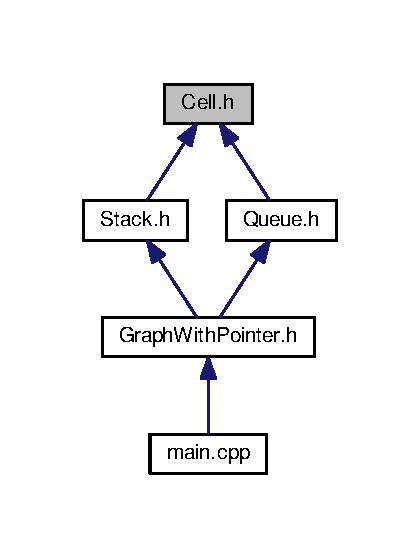
\includegraphics[width=350pt]{_cell_8h__dep__incl}
\end{center}
\end{figure}
\subsection*{Clases}
\begin{DoxyCompactItemize}
\item 
class {\bf Cell$<$ D $>$}
\end{DoxyCompactItemize}

\section{Edge.\-h File Reference}
\label{_edge_8h}\index{Edge.\-h@{Edge.\-h}}
{\ttfamily \#include \char`\"{}Node.\-h\char`\"{}}\\*
Include dependency graph for Edge.\-h\-:
\nopagebreak
\begin{figure}[H]
\begin{center}
\leavevmode
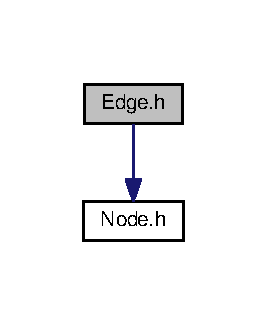
\includegraphics[width=128pt]{_edge_8h__incl}
\end{center}
\end{figure}
This graph shows which files directly or indirectly include this file\-:
\nopagebreak
\begin{figure}[H]
\begin{center}
\leavevmode
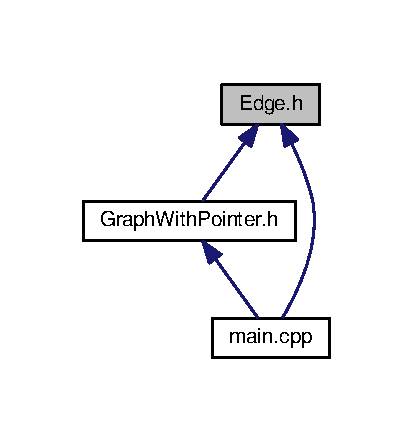
\includegraphics[width=197pt]{_edge_8h__dep__incl}
\end{center}
\end{figure}
\subsection*{Classes}
\begin{DoxyCompactItemize}
\item 
class {\bf Edge$<$ D $>$}
\end{DoxyCompactItemize}

\section{Graph\-With\-Pointer.\-h File Reference}
\label{_graph_with_pointer_8h}\index{Graph\-With\-Pointer.\-h@{Graph\-With\-Pointer.\-h}}
{\ttfamily \#include \char`\"{}Stack.\-h\char`\"{}}\\*
{\ttfamily \#include \char`\"{}Queue.\-h\char`\"{}}\\*
{\ttfamily \#include \char`\"{}Node.\-h\char`\"{}}\\*
{\ttfamily \#include \char`\"{}Edge.\-h\char`\"{}}\\*
{\ttfamily \#include $<$climits$>$}\\*
Include dependency graph for Graph\-With\-Pointer.\-h\-:
\nopagebreak
\begin{figure}[H]
\begin{center}
\leavevmode
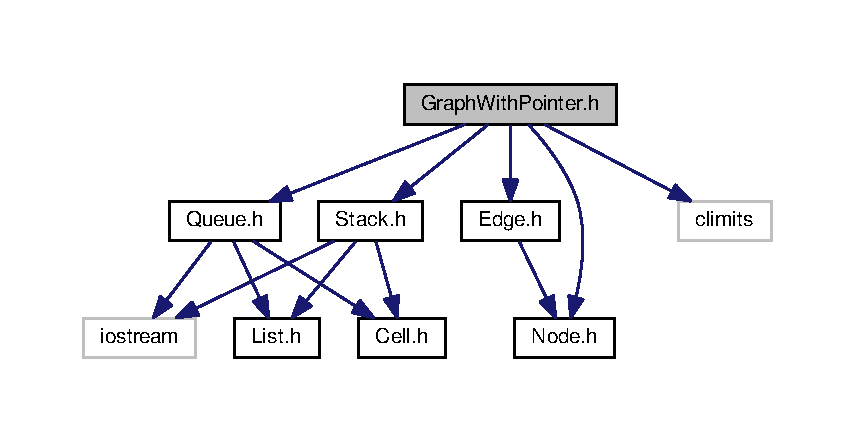
\includegraphics[width=350pt]{_graph_with_pointer_8h__incl}
\end{center}
\end{figure}
This graph shows which files directly or indirectly include this file\-:
\nopagebreak
\begin{figure}[H]
\begin{center}
\leavevmode
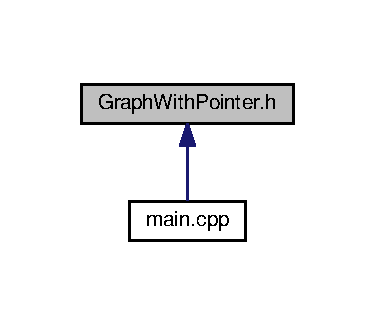
\includegraphics[width=180pt]{_graph_with_pointer_8h__dep__incl}
\end{center}
\end{figure}
\subsection*{Classes}
\begin{DoxyCompactItemize}
\item 
class {\bf Graph\-With\-Pointer$<$ D $>$}
\end{DoxyCompactItemize}

\section{List.\-h File Reference}
\label{_list_8h}\index{List.\-h@{List.\-h}}
This graph shows which files directly or indirectly include this file\-:
\nopagebreak
\begin{figure}[H]
\begin{center}
\leavevmode
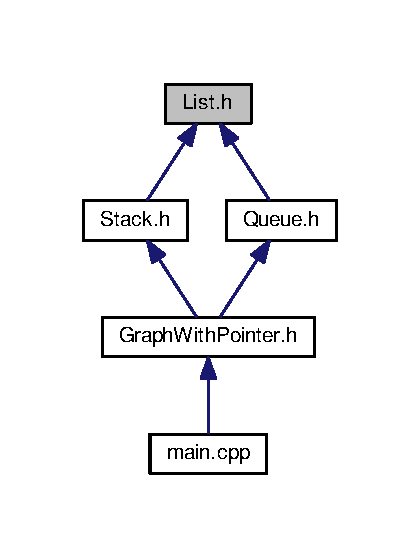
\includegraphics[width=201pt]{_list_8h__dep__incl}
\end{center}
\end{figure}
\subsection*{Classes}
\begin{DoxyCompactItemize}
\item 
class {\bf List$<$ D, P $>$}
\end{DoxyCompactItemize}

\section{Referencia del Archivo main.\-cpp}
\label{main_8cpp}\index{main.\-cpp@{main.\-cpp}}
{\ttfamily \#include $<$iostream$>$}\\*
{\ttfamily \#include \char`\"{}List\-With\-Array.\-h\char`\"{}}\\*
{\ttfamily \#include \char`\"{}List\-With\-Pointer.\-h\char`\"{}}\\*
{\ttfamily \#include \char`\"{}Cell.\-h\char`\"{}}\\*
{\ttfamily \#include \char`\"{}Queue.\-h\char`\"{}}\\*
{\ttfamily \#include \char`\"{}Stack.\-h\char`\"{}}\\*
Dependencia gráfica adjunta para main.\-cpp\-:\nopagebreak
\begin{figure}[H]
\begin{center}
\leavevmode
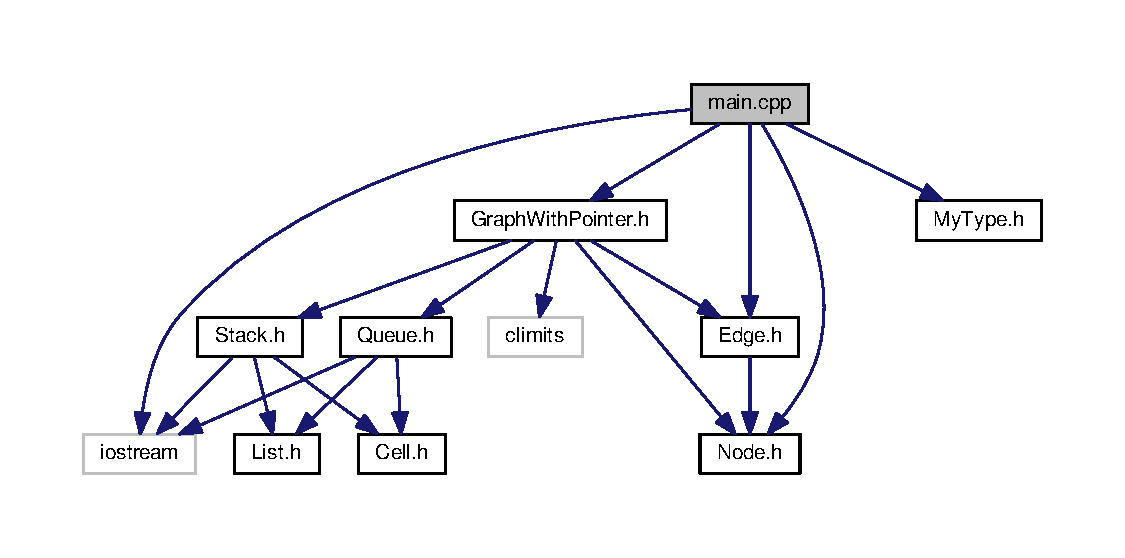
\includegraphics[width=350pt]{main_8cpp__incl}
\end{center}
\end{figure}
\subsection*{Funciones}
\begin{DoxyCompactItemize}
\item 
int {\bf main} (int argc, char $\ast$$\ast$argv)
\end{DoxyCompactItemize}


\subsection{Documentación de las funciones}
\index{main.\-cpp@{main.\-cpp}!main@{main}}
\index{main@{main}!main.cpp@{main.\-cpp}}
\subsubsection[{main}]{\setlength{\rightskip}{0pt plus 5cm}int main (
\begin{DoxyParamCaption}
\item[{int}]{argc, }
\item[{char $\ast$$\ast$}]{argv}
\end{DoxyParamCaption}
)}\label{main_8cpp_a3c04138a5bfe5d72780bb7e82a18e627}


Definición en la línea 9 del archivo main.\-cpp.



Gráfico de llamadas para esta función\-:\nopagebreak
\begin{figure}[H]
\begin{center}
\leavevmode
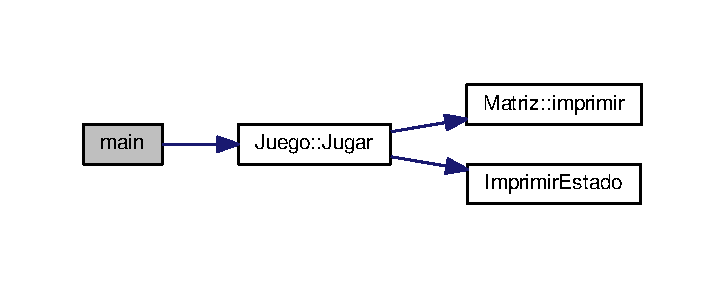
\includegraphics[height=550pt]{main_8cpp_a3c04138a5bfe5d72780bb7e82a18e627_cgraph}
\end{center}
\end{figure}



\section{My\-Type.\-cpp File Reference}
\label{_my_type_8cpp}\index{My\-Type.\-cpp@{My\-Type.\-cpp}}
{\ttfamily \#include \char`\"{}My\-Type.\-h\char`\"{}}\\*
Include dependency graph for My\-Type.\-cpp\-:
\nopagebreak
\begin{figure}[H]
\begin{center}
\leavevmode
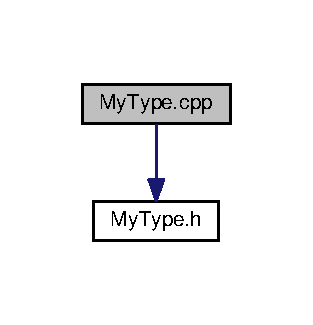
\includegraphics[width=150pt]{_my_type_8cpp__incl}
\end{center}
\end{figure}

\section{My\-Type.\-h File Reference}
\label{_my_type_8h}\index{My\-Type.\-h@{My\-Type.\-h}}
This graph shows which files directly or indirectly include this file\-:
\nopagebreak
\begin{figure}[H]
\begin{center}
\leavevmode
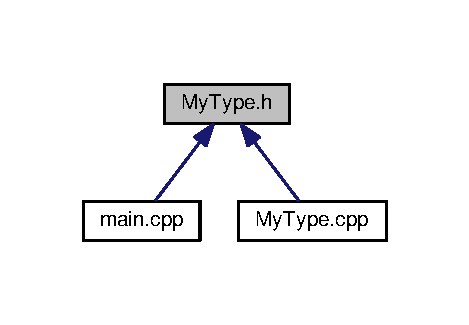
\includegraphics[width=225pt]{_my_type_8h__dep__incl}
\end{center}
\end{figure}
\subsection*{Classes}
\begin{DoxyCompactItemize}
\item 
class {\bf My\-Type}
\begin{DoxyCompactList}\small\item\em Clase \doxyref{My\-Type}{p.}{class_my_type}. \end{DoxyCompactList}\end{DoxyCompactItemize}

\section{Node.\-h File Reference}
\label{_node_8h}\index{Node.\-h@{Node.\-h}}
This graph shows which files directly or indirectly include this file\-:
\nopagebreak
\begin{figure}[H]
\begin{center}
\leavevmode
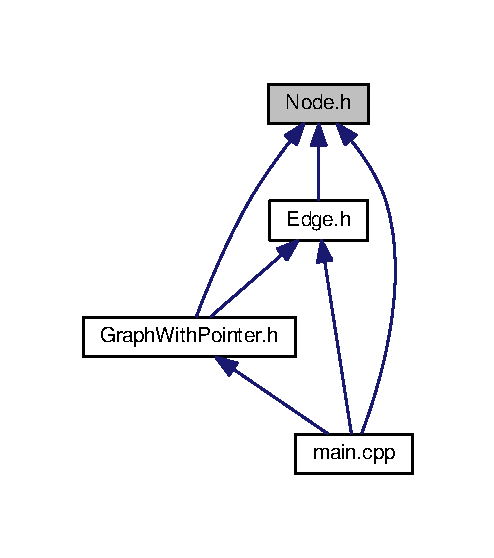
\includegraphics[width=237pt]{_node_8h__dep__incl}
\end{center}
\end{figure}
\subsection*{Classes}
\begin{DoxyCompactItemize}
\item 
class {\bf Edge$<$ D $>$}
\item 
class {\bf Node$<$ D $>$}
\end{DoxyCompactItemize}

\section{Referencia del Archivo Queue.\-h}
\label{_queue_8h}\index{Queue.\-h@{Queue.\-h}}
{\ttfamily \#include $<$iostream$>$}\\*
{\ttfamily \#include \char`\"{}List.\-h\char`\"{}}\\*
{\ttfamily \#include \char`\"{}Cell.\-h\char`\"{}}\\*
Dependencia gráfica adjunta para Queue.\-h\-:\nopagebreak
\begin{figure}[H]
\begin{center}
\leavevmode
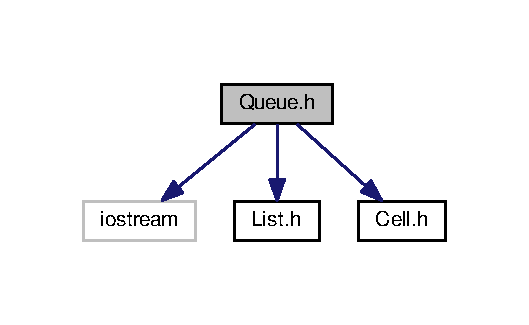
\includegraphics[width=254pt]{_queue_8h__incl}
\end{center}
\end{figure}
Gráfico de los archivos que directa o indirectamente incluyen a este archivo\-:\nopagebreak
\begin{figure}[H]
\begin{center}
\leavevmode
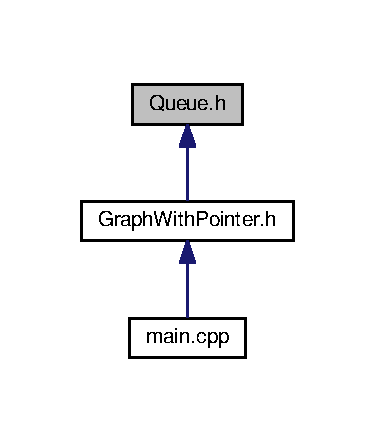
\includegraphics[width=134pt]{_queue_8h__dep__incl}
\end{center}
\end{figure}
\subsection*{Clases}
\begin{DoxyCompactItemize}
\item 
class {\bf Queue$<$ D, P $>$}
\end{DoxyCompactItemize}

\section{Stack.\-h File Reference}
\label{_stack_8h}\index{Stack.\-h@{Stack.\-h}}
{\ttfamily \#include $<$iostream$>$}\\*
{\ttfamily \#include \char`\"{}List.\-h\char`\"{}}\\*
{\ttfamily \#include \char`\"{}Cell.\-h\char`\"{}}\\*
Include dependency graph for Stack.\-h\-:
\nopagebreak
\begin{figure}[H]
\begin{center}
\leavevmode
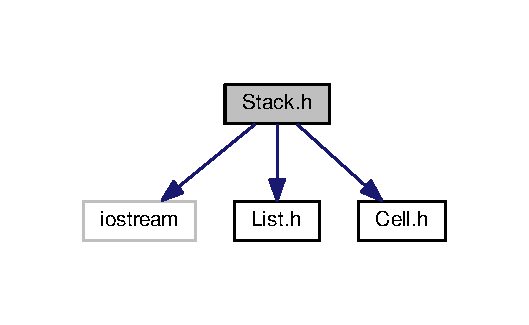
\includegraphics[width=254pt]{_stack_8h__incl}
\end{center}
\end{figure}
This graph shows which files directly or indirectly include this file\-:
\nopagebreak
\begin{figure}[H]
\begin{center}
\leavevmode
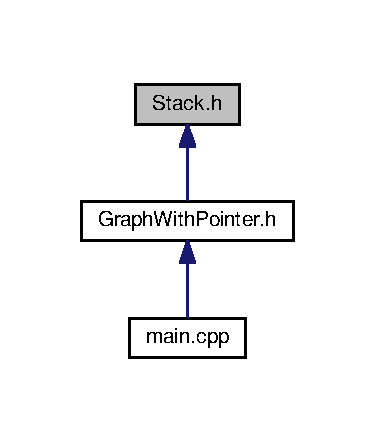
\includegraphics[width=180pt]{_stack_8h__dep__incl}
\end{center}
\end{figure}
\subsection*{Classes}
\begin{DoxyCompactItemize}
\item 
class {\bf Stack$<$ D, P $>$}
\end{DoxyCompactItemize}

%--- End generated contents ---

% Index
\newpage
\phantomsection
\addcontentsline{toc}{chapter}{Index}
\printindex

\end{document}
